\section{Исследование свойств многоканальной системы}
\subsection{Анализ системы}
Рассмотрим систему
\begin{equation}
    \label{eq:sys1}
    \begin{cases}
        \dot x=Ax+Bu\\
        y=Cx
    \end{cases},\quad
    A=\begin{bmatrix}
        0 & 1 \\
        1 & 1
        \end{bmatrix},\quad
        B=\begin{bmatrix}
        1 & 2 \\
        1 & 4
        \end{bmatrix},\quad
        C=\begin{bmatrix}
        2 & -1 \\
        1 & -4
    \end{bmatrix}.
\end{equation}
Спектр $A$
\begin{equation*}
    \sigma(A)=\{-0.6180,\ 1.6180\}
\end{equation*}
Передаточная матрица системы \eqref{eq:sys1}:
\begin{equation*}
    \underset{u\rightarrow y}{W}(s)=\begin{bmatrix}
        -\dfrac{1.0\,{\left(s-1.0\right)}}{-1.0\,s^2 +s+1.0} & -\dfrac{2.0}{-1.0\,s^2 +s+1.0}\\[2ex]
        \dfrac{3.0\,s+4.0}{-1.0\,s^2 +s+1.0} & \dfrac{2.0\,{\left(7.0\,s+3.0\right)}}{-1.0\,s^2 +s+1.0}
    \end{bmatrix}.
\end{equation*}
Нули и полюса определяем из определителя передаточной матрицы:
\begin{equation*}
    \emptyset,\quad \left(\begin{array}{c}
-0.618\\
1.618
\end{array}\right)
\end{equation*}
Как можно видеть, нули идентичны спектру матрицы системы $A$.
Посмотрим на матрицы управляемости по состоянию, по выходу и наблюдаемости:
\begin{equation*}
    U=\begin{bmatrix}
        1 & 2 & 1 & 4 \\
        1 & 4 & 2 & 6
        \end{bmatrix},\quad
        U_\text{вых}=\begin{bmatrix}
        1 & 0 & 0 & 2 & 0 & 0 \\
        -3 & -14 & -7 & -20 & 0 & 0
        \end{bmatrix},\quad
        V=\begin{bmatrix}
        2 & -1 \\
        1 & -4 \\
        -1 & 1 \\
        -4 & -3
    \end{bmatrix}.
\end{equation*}
У них всех ранг равен двум, это значит, что система управляема по состоянию и по выходы, а
так же наблюдаема, как следствие, система стабилизируема и обнаруживаема.
\subsection{Весовая и переходная характеристики}
Получим выражениу для временной весовой характеристики, для этого сначала разложим ПФ
на простые множители:
\begin{equation*}
    \underset{u\rightarrow y}{W}(s)=\begin{bmatrix}
        \dfrac{0.7236}{s+0.618}+\dfrac{0.2764}{s-1.618} &
        \dfrac{0.8944}{s-1.618}-\dfrac{0.8944}{s+0.618} \\[2ex]
        \dfrac{0.9597}{s+0.618}-\dfrac{3.96}{s-1.618} &
        -\dfrac{1.186}{s+0.618}-\dfrac{12.81}{s-1.618}
    \end{bmatrix},
\end{equation*}
значит
\begin{equation*}
    \underset{u\rightarrow y}{w}(t)=\begin{bmatrix}
        0.7236\exp(-0.618t)+0.2764\exp(0.618t) &
        0.8944\exp(0.618t)-0.8944\exp(-0.618t) \\[2ex]
        0.9597\exp(-0.618t)-3.96\exp(0.618t) &
        -1.186\exp(-0.618t)-12.81\exp(0.618t)
    \end{bmatrix}.
\end{equation*}
Графическое представление можно увидеть на рисунке \ref{fig:1_ir}.

\begin{figure}[H]
    \centering
    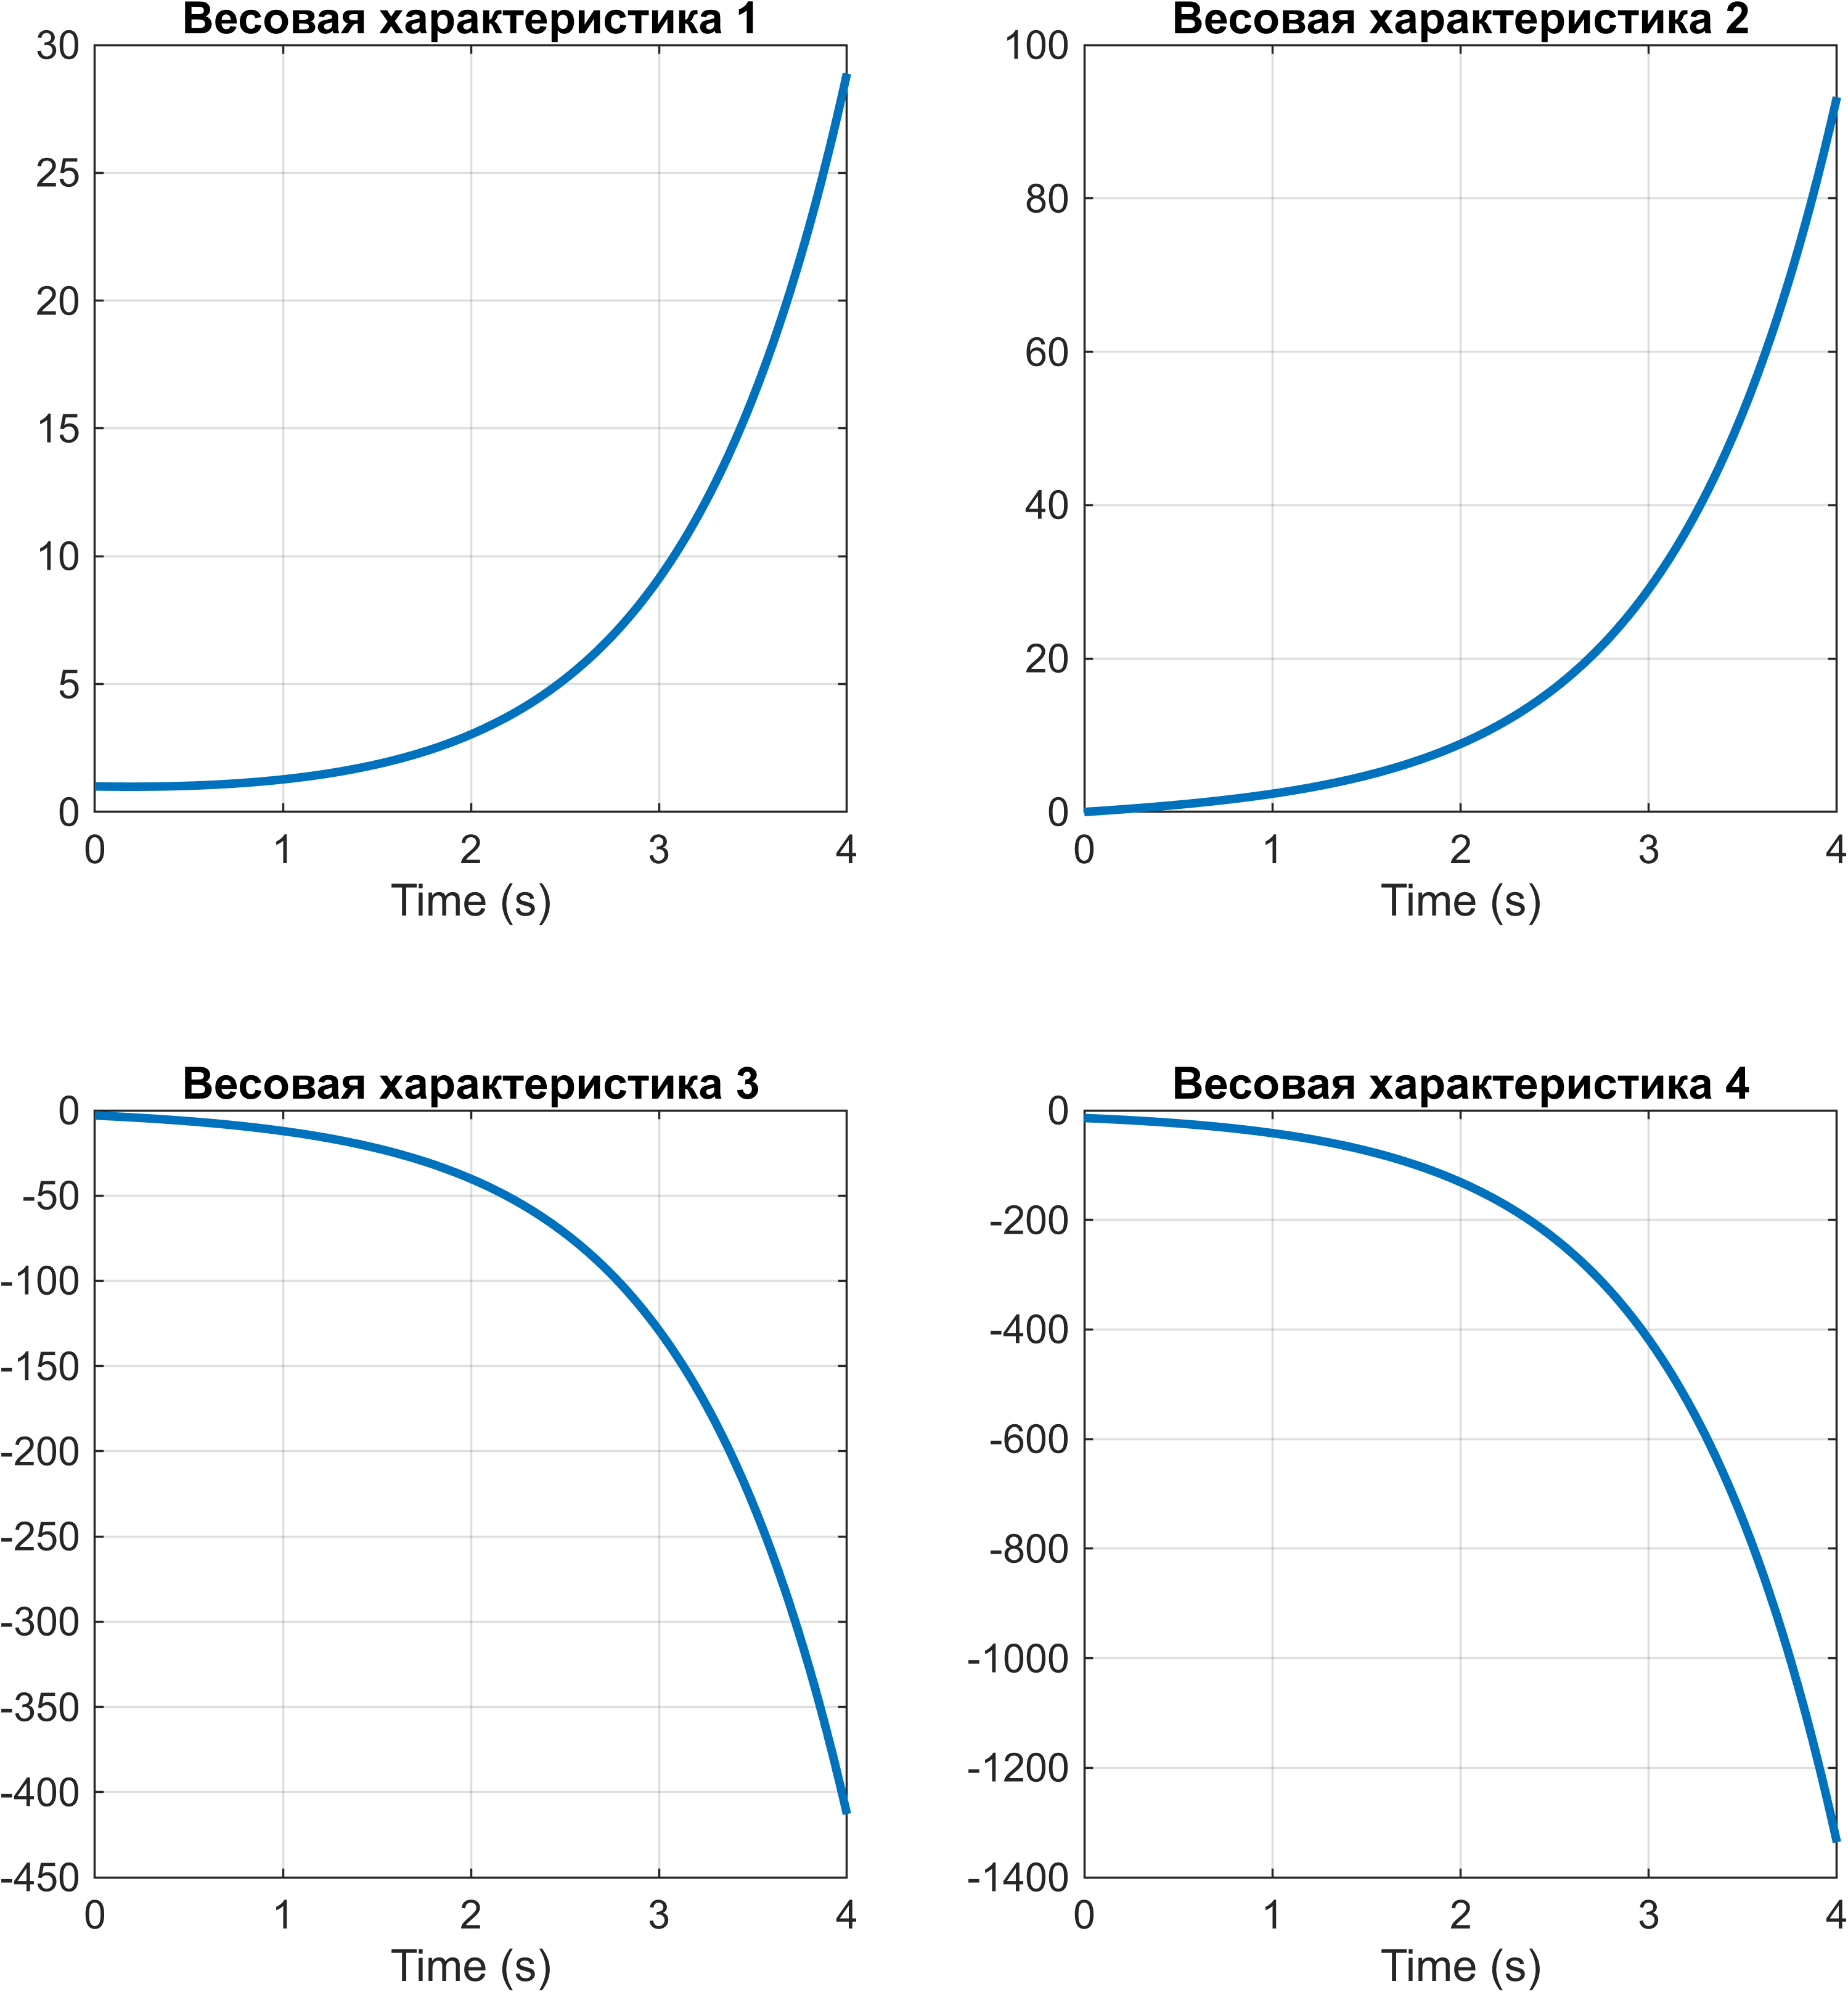
\includegraphics[width=\linewidth]{figs/1_ir.png}
    \caption{Графики весовых характеристик}
    \label{fig:1_ir}
\end{figure}

\noindent Аналогичным образом получим переходную характеристику 
$y_{s.r.}=\mathcal{L}^{-1}\left( \frac{W(s)}{s} \right)$:
\begin{equation*}
    y_{s.r.}=\begin{bmatrix}
        0.1708\,{\mathrm{e}}^{1.162\,t} -1.171\,{\mathrm{e}}^{-0.618\,t} +1.0 &
        0.5528\,{\mathrm{e}}^{1.162\,t} +1.447\,{\mathrm{e}}^{-0.618\,t} -2.0 \\
        4.0-1.553\,{\mathrm{e}}^{-0.618\,t} -2.447\,{\mathrm{e}}^{1.162\,t} &
        1.919\,{\mathrm{e}}^{-0.618\,t} -7.919\,{\mathrm{e}}^{1.162\,t} +6.0
    \end{bmatrix}
\end{equation*}
Графическое представление можно увидеть на рисунке \ref{fig:1_sr}.
\begin{figure}[H]
    \centering
    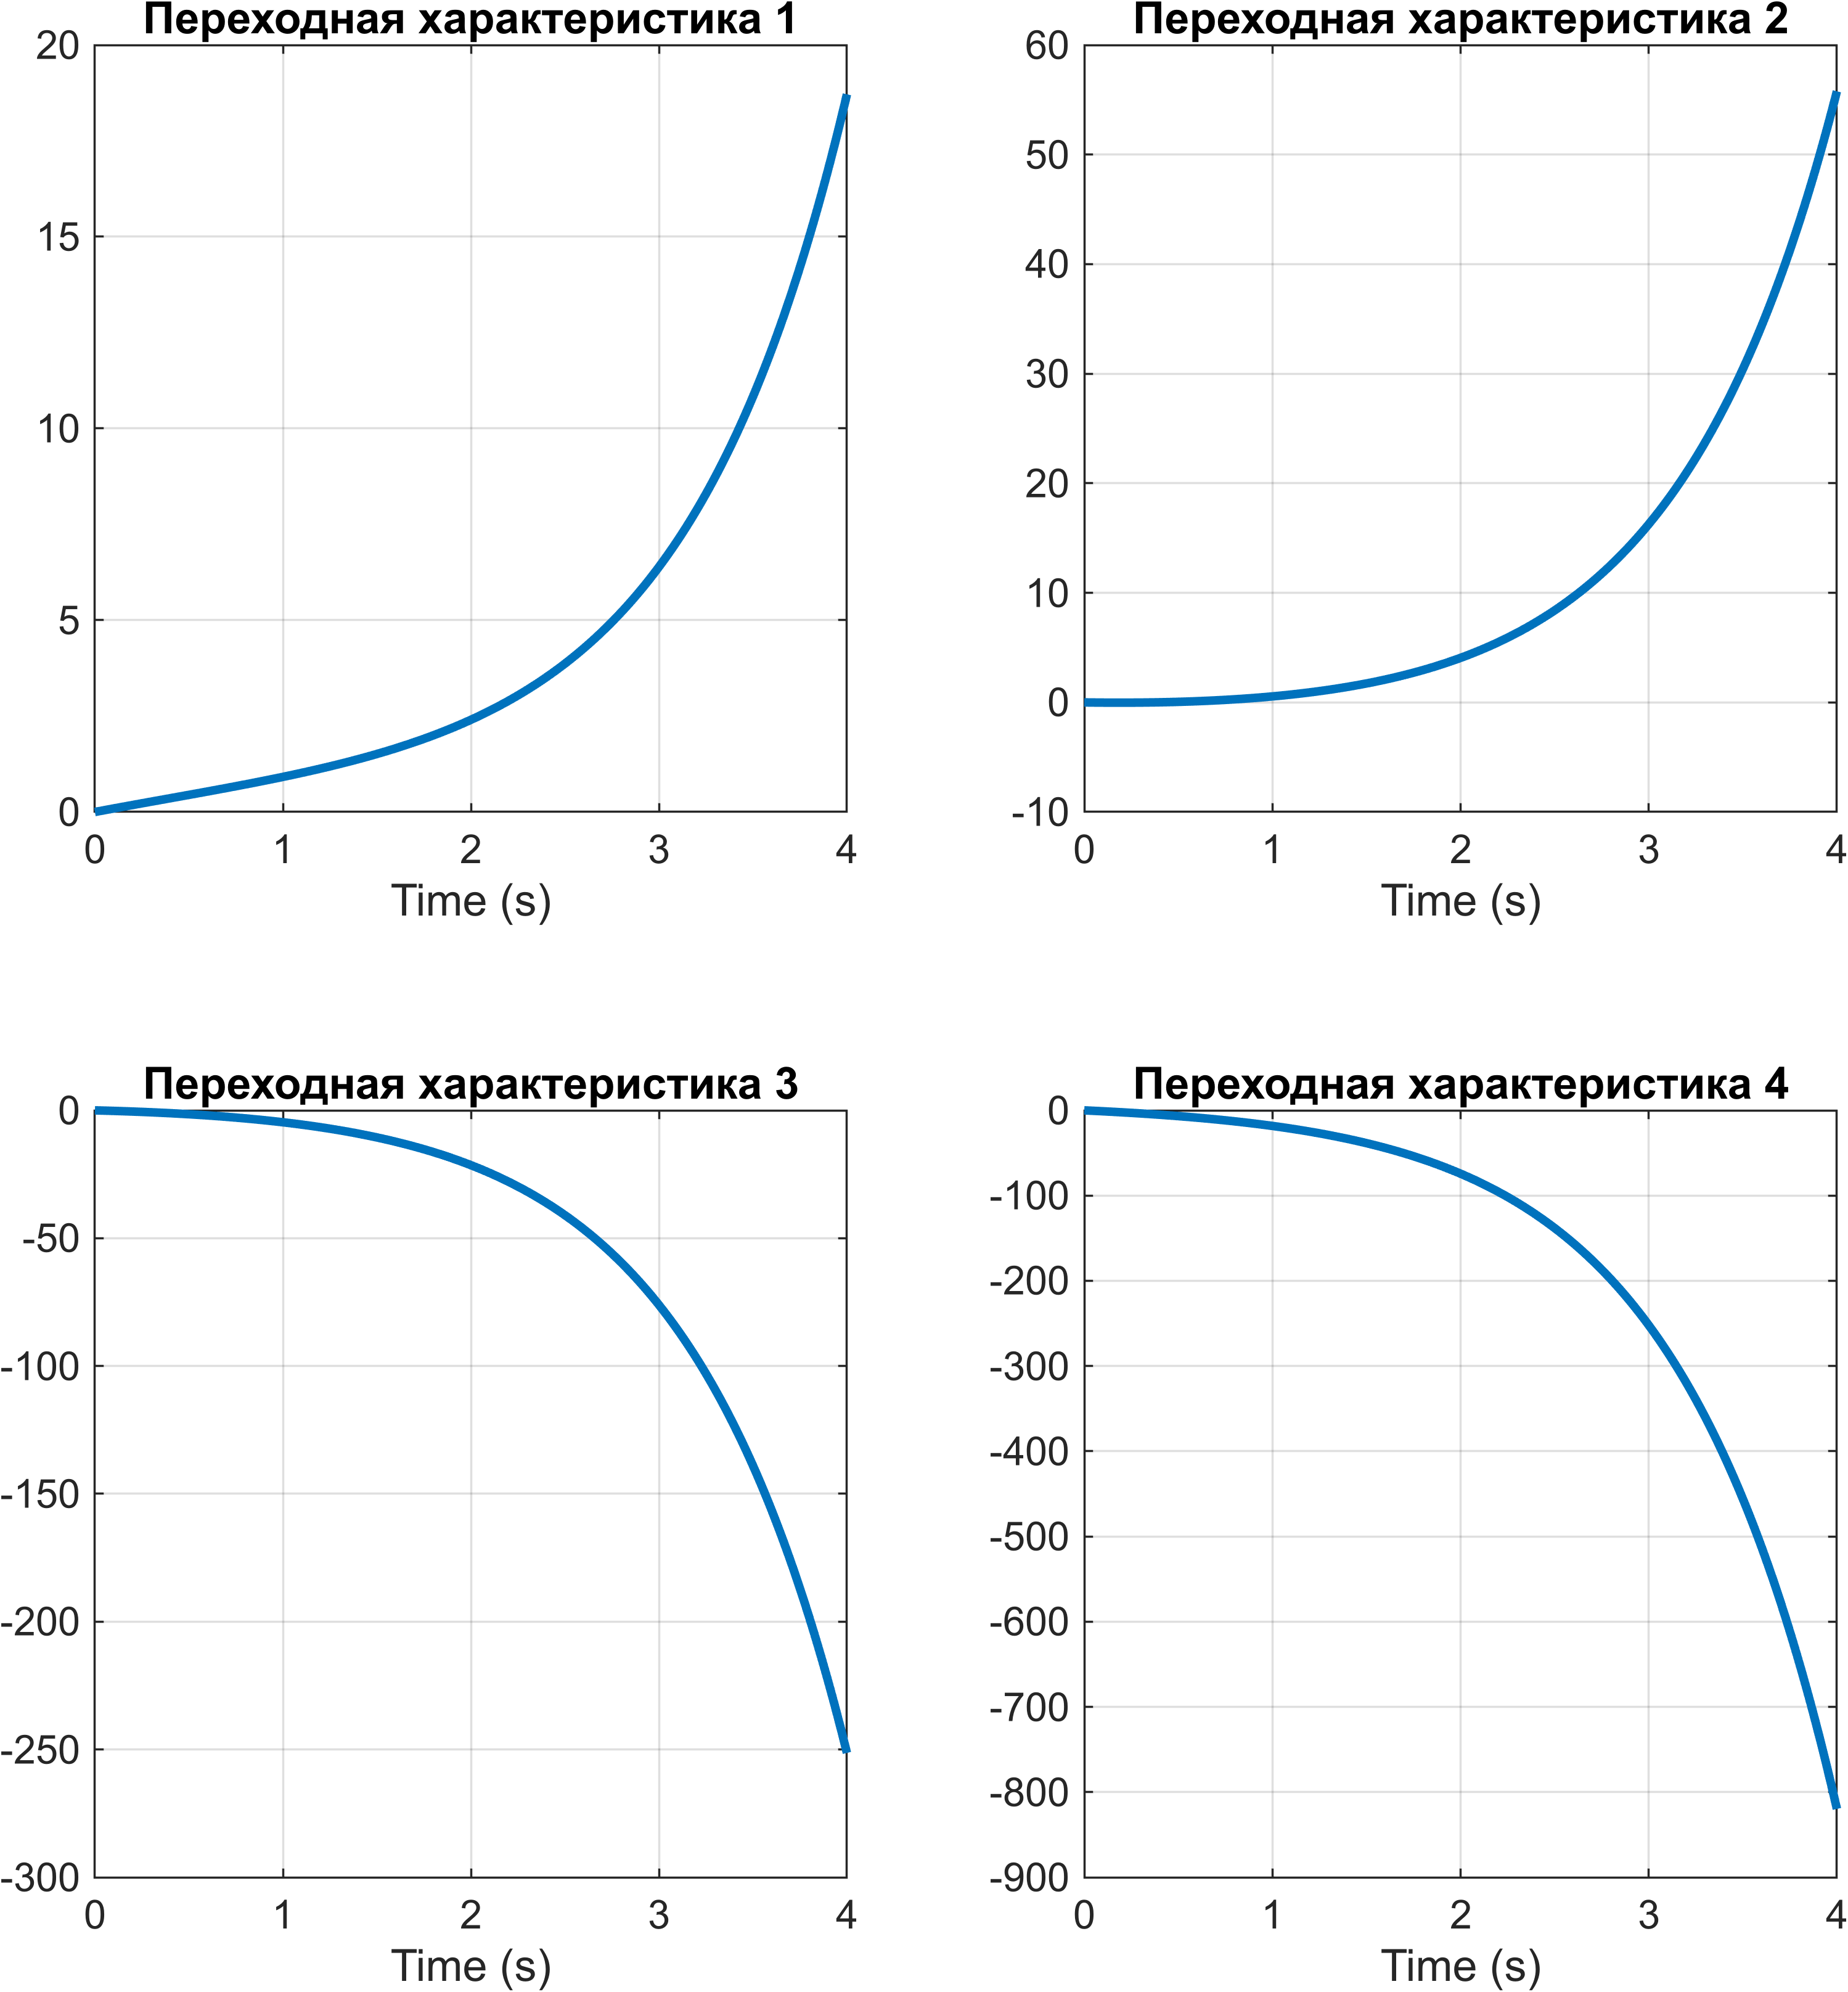
\includegraphics[width=\linewidth]{figs/1_sr.png}
    \caption{Графики переходных характеристик}
    \label{fig:1_sr}
\end{figure}
\subsection{Частотные характеристики}
Подставим $i\omega$ в передаточную матрицу:
\begin{equation*}
    W(i\omega)=
    \begin{bmatrix}
        -\dfrac{\omega^3 \,\mathrm{i}+2\,\omega \,\mathrm{i}-1}{\omega^4 +3\,\omega^2 +1 } & 
        -\dfrac{2\,\omega^2 -2\,\omega \,\mathrm{i}+2}{\omega^4 +3\,\omega^2 +1 }\\[2ex]
        \dfrac{3\,\omega^3 \,\mathrm{i}+7\,\omega^2 -\omega \,\mathrm{i}+4}{\omega^4 +3\,\omega^2 +1 } & 
        \dfrac{14\,\omega^3 \,\mathrm{i}+20\,\omega^2 +8\,\omega \,\mathrm{i}+6}{\omega^4 +3\,\omega^2 +1 }
    \end{bmatrix}
\end{equation*}
и получим функции АЧХ 
$$A_i(\omega)=\sqrt{\mathbf{Re}(W_i(i\omega))^2+\mathbf{Im}(W_i(i\omega))^2},$$
ФЧХ
$$\varphi_i(\omega)=\text{atan2}\left( \mathbf{Im}(W_i(i\omega)),\ \mathbf{Re}(W_i(i\omega)) \right)$$
и ЛАЧХ:
$$L_i(\omega)=20\log_{10}A_i(\omega).$$
Вычислим их:
\begin{equation*}
    A(\omega)=
\begin{bmatrix}
\dfrac{\sqrt{{\left|\omega \right|}^2 \,{{\left(\omega^2 +2.0\right)}}^2 +1.0}}{\omega^4 +3\,\omega^2 +1 } & 
\dfrac{2.0}{\sqrt{\omega^4 +3\,\omega^2 +1 }} \\[2ex]
\dfrac{\sqrt{9.0\,\omega^6 +43.0\,\omega^4 +57.0\,\omega^2 +16.0}}{\omega^4 +3\,\omega^2 +1 } & 
\dfrac{2.0\,\sqrt{49.0\,\omega^2 +9.0}}{\sqrt{\omega^4 +3\,\omega^2 +1 }}
\end{bmatrix},
\end{equation*}
\begin{equation*}
    \varphi(\omega)=\begin{bmatrix}
\textrm{atan2}\left(1.0,-1.0\,\omega^3 -2.0\,\omega \right) & 
\textrm{atan2}\left(-1.0\,\omega^2 -1.0,\omega \right) \\[2ex]
\textrm{atan2}\left(7.0\,\omega^2 +4.0,\omega \,{\left(3.0\,\omega^2 -1.0\right)}\right) &
\textrm{atan2}\left(\dfrac{1.0\,{\left(10.0\,\omega^2 +3.0\right)}}{7.0\,\omega^2 +4.0},\omega \right)
\end{bmatrix},
\end{equation*}
\begin{equation*}
    L(\omega)=
    8.686\cdot\begin{bmatrix}
\log \left(\dfrac{\sqrt{{\left|\omega \right|}^2 \,{{\left(\omega^2 +2.0\right)}}^2 +1.0}}{\omega^4 +3.0\,\omega^2 +1.0 }\right) & 
\log \left(\dfrac{2.0}{\sqrt{\omega^4 +3.0\,\omega^2 +1.0 }}\right) \\[2ex]
\log \left(\dfrac{\sqrt{9.0\,\omega^6 +43.0\,\omega^4 +57.0\,\omega^2 +16.0}}{\omega^4 +3.0\,\omega^2 +1.0 }\right) &
\log \left(\dfrac{2.0\,\sqrt{49.0\,\omega^2 +9.0}}{\sqrt{\omega^4 +3.0\,\omega^2 +1.0 }}\right)
\end{bmatrix}
\end{equation*}
Графики АЧХ и ФЧХ можно увидеть на рисунке \ref{fig:1_freq}, ЛАЧХ и ЛФЧХ
на рисунке \ref{fig:1_logfreq}.
\begin{figure}[H]
    \centering
    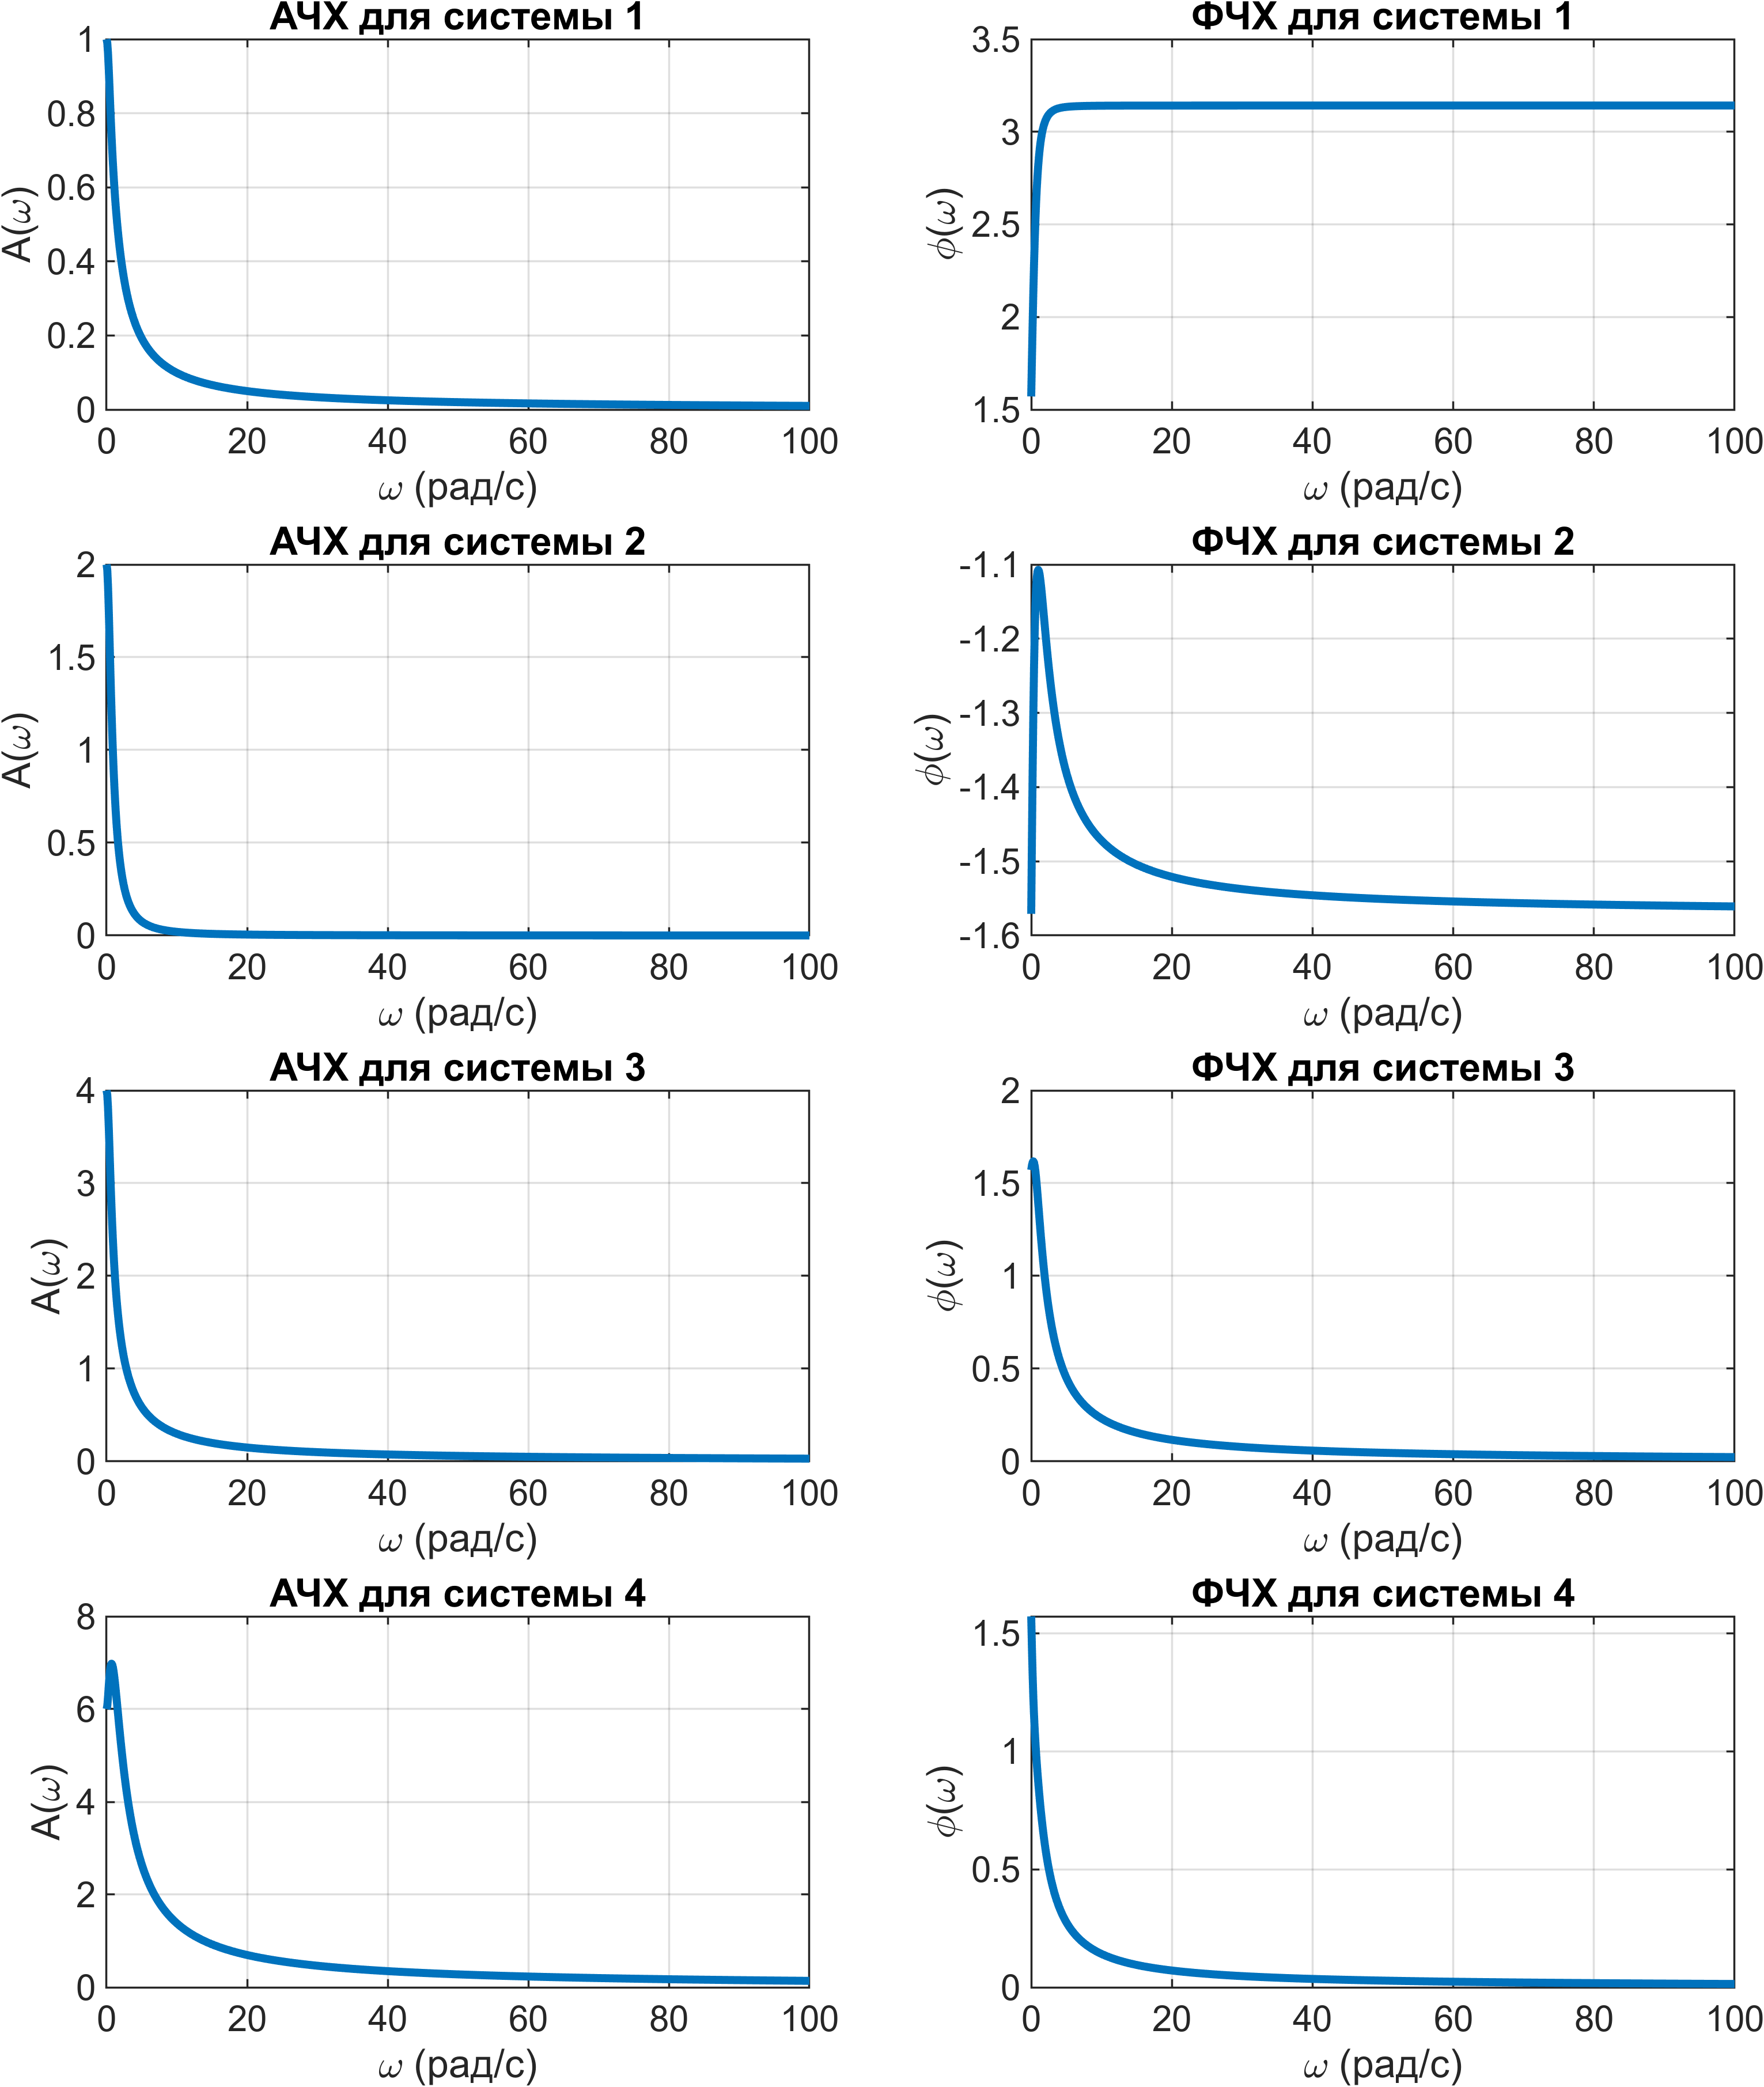
\includegraphics[width=\linewidth]{figs/combined_A_P_freq.png}
    \caption{АЧХ и ФЧХ}
    \label{fig:1_freq}
\end{figure}
\begin{figure}[H]
    \centering
    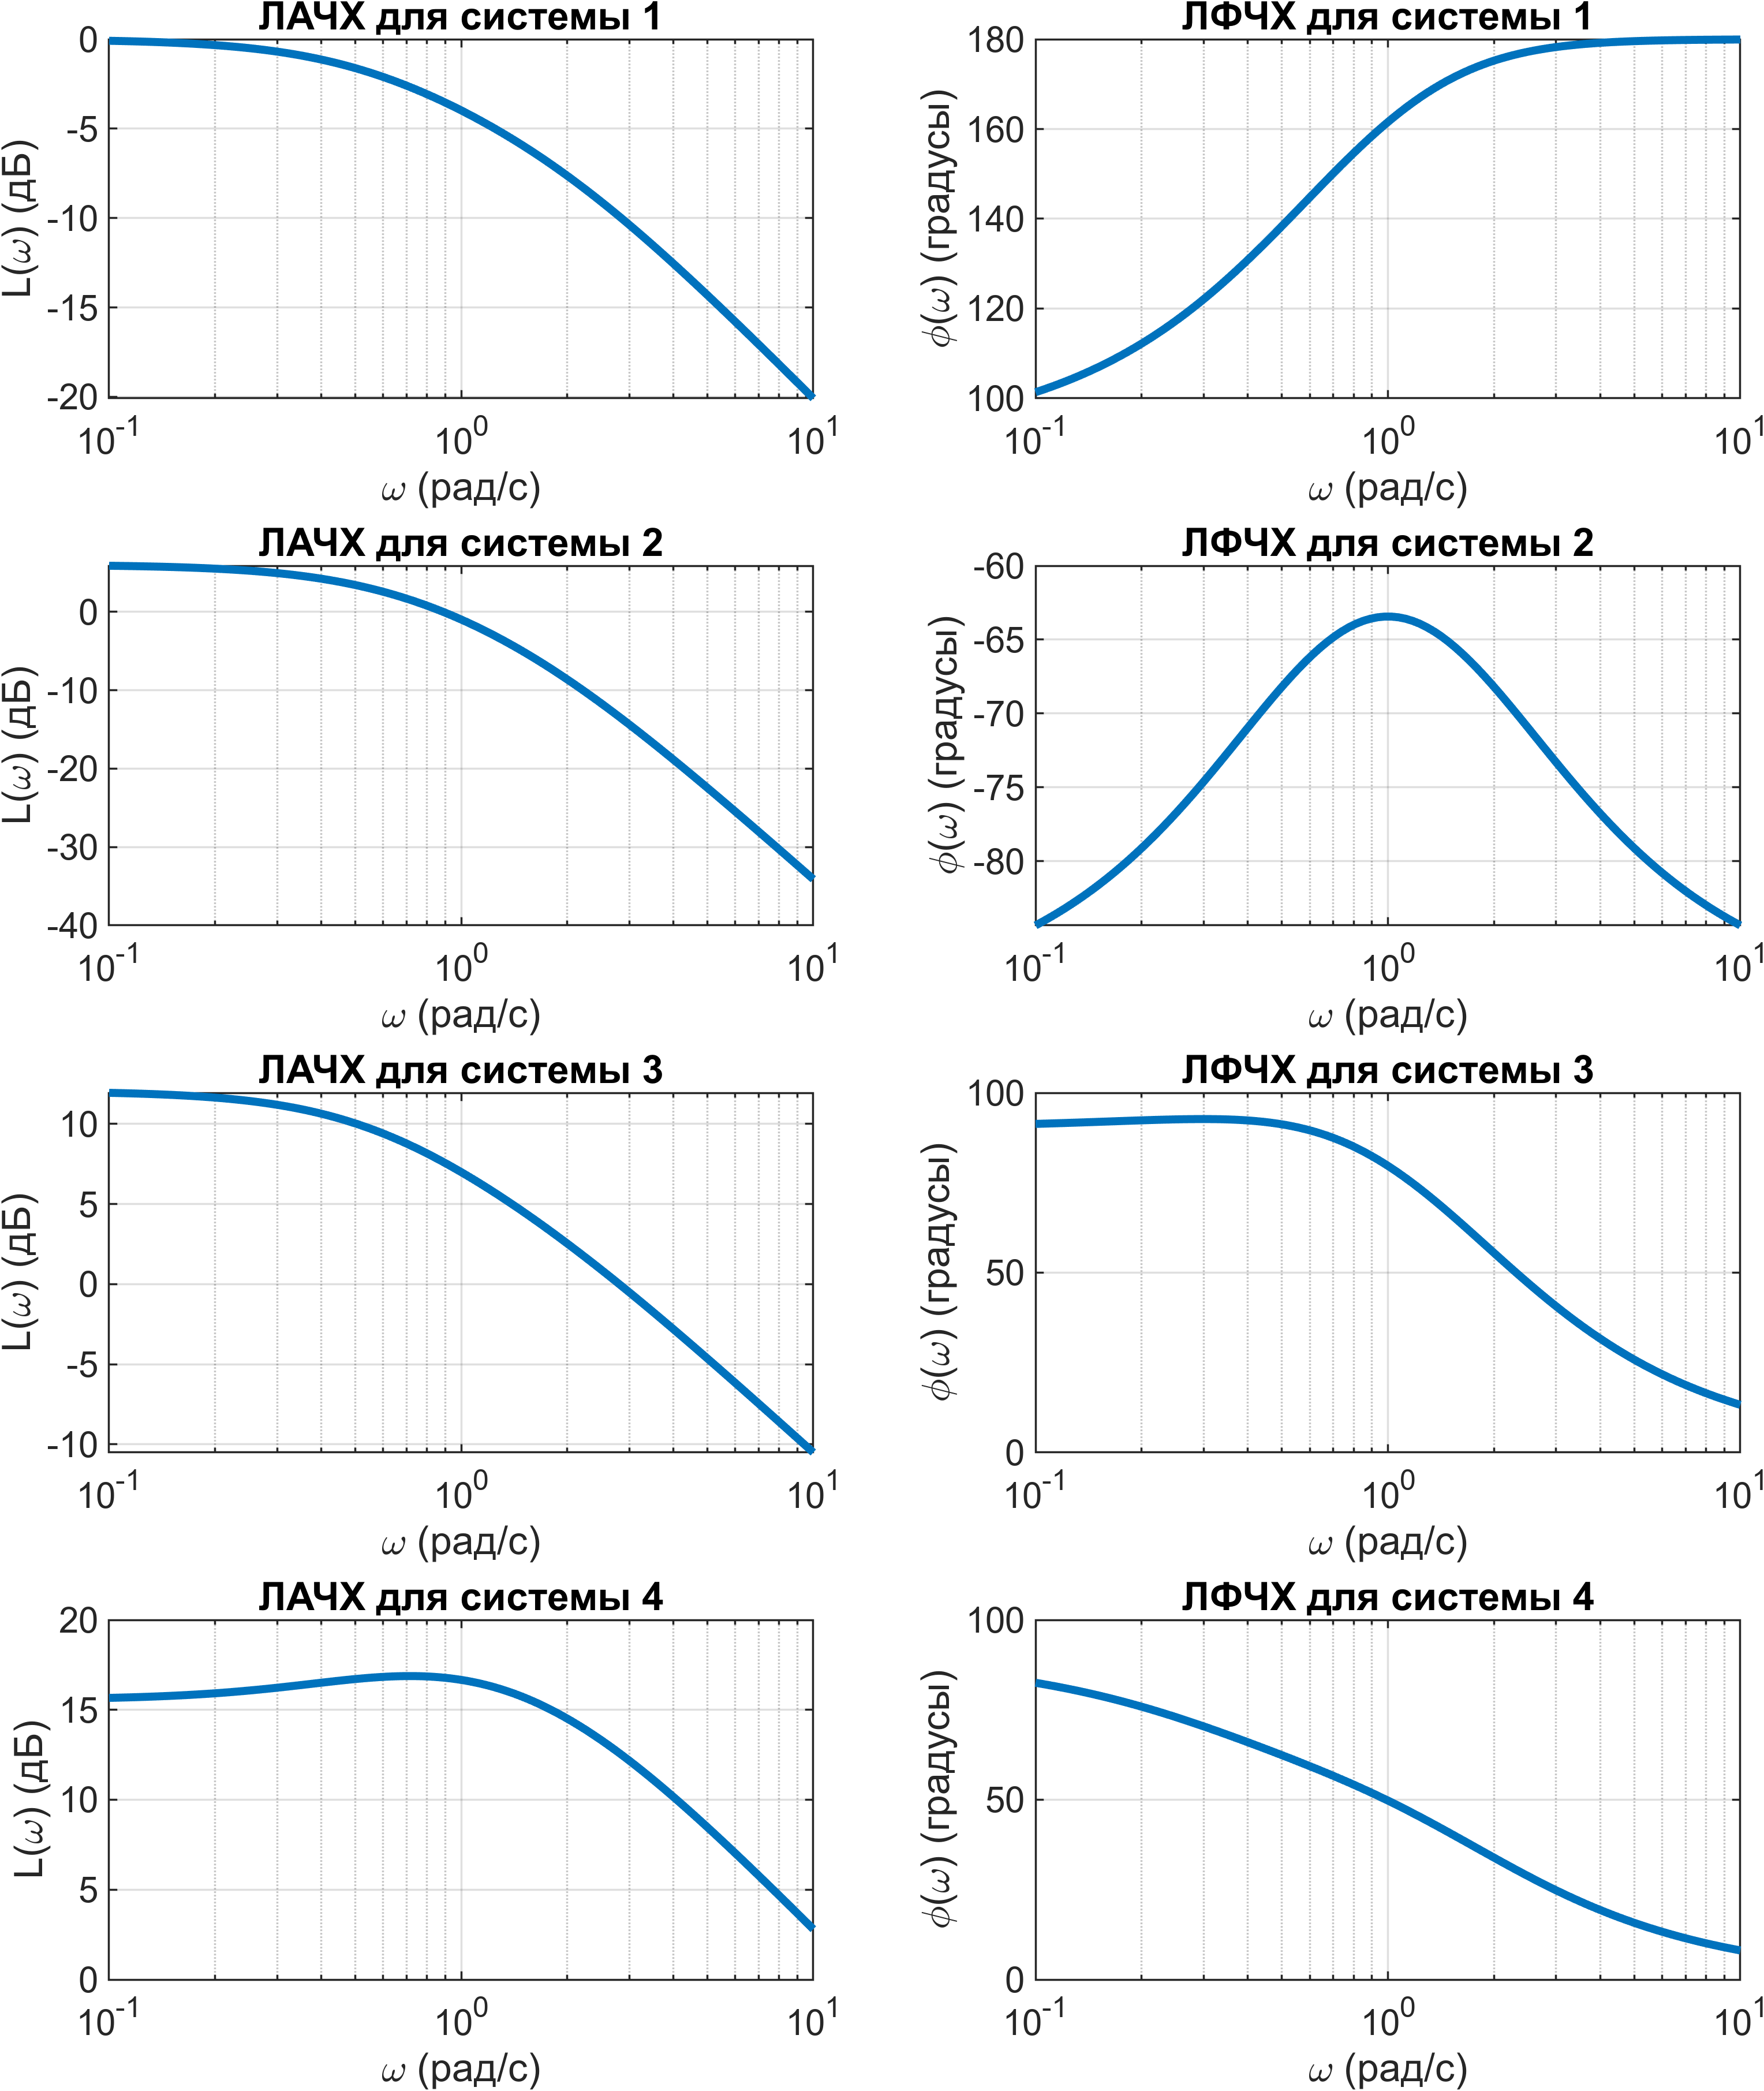
\includegraphics[width=\linewidth]{figs/combined_L_P_logfreq.png}
    \caption{ЛАЧХ и ЛФЧХ}
    \label{fig:1_logfreq}
\end{figure}

\subsection{Выводы}

В результате проведённого анализа многоканальной системы установлено, 
что система является полностью управляемой, как по состоянию, так и по управлению, 
и наблюдаемой, а следовательно, стабилизируемой и обнаруживаемой. Матрица системы
является неустойчивой, что подтвердается полученными временными характеристиками: 
весовыми и переходными; также были получены 
частотные характеристики: АЧХ, ФЧХ, ЛАЧХ и ЛФЧХ. 


\section{Синтез следящего управления в условиях внешних 
возмущений для многоканальной системы}
\subsection{Анализ системы}
\label{sec:anal}
Рассмотрим систему
\begin{equation}
    \label{eq:sys2}
    \begin{cases}
        \dot x=Ax+Bu+B_ff_1\\
        z=C_zx+D_zu-g\\
        y=Cx+Du+D_ff_2
    \end{cases},\quad
    x(0)=\begin{bmatrix}
        1\\1
    \end{bmatrix},
\end{equation}
где
\begin{equation*}
    A=\begin{bmatrix}
        0&1\\1&1
    \end{bmatrix},\quad
    B=\begin{bmatrix}
        1&2\\1&4
    \end{bmatrix},\quad
    B_f=\begin{bmatrix}
        1&2\\-2&4
    \end{bmatrix}
\end{equation*}
\begin{equation*}
    C=\begin{bmatrix}
        2&-1\\1&-4
    \end{bmatrix},\quad
    D=\begin{bmatrix}
        1&0\\0&-1
    \end{bmatrix},\quad
    D_f=\begin{bmatrix}
        -1&0\\0&1
    \end{bmatrix},
\end{equation*}
\begin{equation*}
    C_z=\begin{bmatrix}
        3&1\\-2&4
    \end{bmatrix},\quad
    D_z=\begin{bmatrix}
        1&0\\0&1
    \end{bmatrix},
\end{equation*}
\begin{equation*}
    f_1(t)=\begin{bmatrix}
        3\cos(t)\\11\sin(3t)
    \end{bmatrix},\quad
    f_2(t)=\begin{bmatrix}
        \sin(3t)\\8\cos(t)
    \end{bmatrix},\quad
    g(t)=\begin{bmatrix}
        3\cos(6t)\\\sin(6t)
    \end{bmatrix}.
\end{equation*}
Считаем доступными к измерению только величины $y(t)$ и $g(t)$.
Посмотрим на матрицу управляемости по состоянию:
\begin{equation*}
    U=\begin{bmatrix}
        1 & 2 & 1 & 4 \\
        1 & 4 & 2 & 6
    \end{bmatrix}.
\end{equation*}
Ранг равен двум, значит, система управляема по состоянию, как следствие, 
система стабилизируема.
Посмотрим на матрицы наблюдаемости относительно $y$ и $z$:
\begin{equation*}
    V_y=\begin{bmatrix}
        2 & -1 \\
        1 & -4 \\
        -1 & 1 \\
        -4 & -3
    \end{bmatrix},\quad
    V_z=\begin{bmatrix}
        3&	1\\
        -2&	4\\
        1	&4\\
        4	&2
    \end{bmatrix}.
\end{equation*}
Обе матрицы имеют ранг два, следовательно относительно них система наблюдаема и,
как следствие, обнаруживаема.
Посмотрим на матрицы управляемости по выходу относительно $y$ и $z$:
\begin{equation*}
    U_y=\begin{bmatrix}
        1&	0&	0	&2&	1&0\\
        -3	&-14	&-7&	-20&	0&	-1
    \end{bmatrix},\quad
    U_z=\begin{bmatrix}
        1&	0&	0	&2&	1&0\\
        -3	&-14	&-7&	-20&	0&	1
    \end{bmatrix}.
\end{equation*}
Обе матрицы имеют ранг два, следовательно относительно них система управляема.
Передаточная матрица от $u$ к $y$ и ее определитель:
\begin{equation*}
    \underset{u\rightarrow y}{W}(s)=\begin{bmatrix}
-\dfrac{s^2 -2}{-s^2 +s+1} & -\dfrac{2}{-s^2 +s+1}\\[2ex]
\dfrac{3\,s+4}{-s^2 +s+1} & \dfrac{s^2 +13\,s+5}{-s^2 +s+1}
\end{bmatrix},\quad
\Delta\underset{u\rightarrow y}{W}(s)=\frac{s^2 +14\,s+18}{-s^2 +s+1},
\end{equation*}
как видно, передаточная матрица невырождена.
Передаточная матрица от $u$ к $z$ и ее определитель:
\begin{equation*}
    \underset{u\rightarrow z}{W}(s)=\begin{bmatrix}
-\dfrac{s\,{\left(s+3\right)}}{-s^2 +s+1} & -\dfrac{2\,{\left(5\,s+4\right)}}{-s^2 +s+1}\\[2ex]
-\dfrac{2\,{\left(s+2\right)}}{-s^2 +s+1} & -\dfrac{s^2 +11\,s+3}{-s^2 +s+1}
\end{bmatrix},\quad
\Delta\underset{u\rightarrow z}{W}(s)=-\frac{s^2 +15\,s+32}{-s^2 +s+1},
\end{equation*}
как видно, эта передаточная матрица тоже невырождена.
Определим матрицы и начальные условия генератора внешнего воздействия:
\begin{equation}
    \label{eq:gen}
    \begin{cases}
        \dot w=\Gamma_ww\\
        g=Y_gw\\
        f_1=Y_1w\\
        f_2=Y_2w
    \end{cases},\quad
    w(0).
\end{equation}
\begin{equation*}
    \Gamma_w=\begin{bmatrix}
        0 & -6 & 0 & 0 & 0 & 0\\
        6 & 0 & 0 & 0 & 0 & 0\\
        0 & 0 & 0 & -1 & 0 & 0\\
        0 & 0 & 1 & 0 & 0 & 0\\
        0 & 0 & 0 & 0 & 0 & -3\\
        0 & 0 & 0 & 0 & 3 & 0
    \end{bmatrix},\quad
    Y_g=\begin{bmatrix}
        \frac{3}{2} & -\frac{1}{2}\\
        \frac{3}{2} & \frac{1}{2}\\
        0 & 0\\
        0 & 0\\
        0 & 0\\
        0 & 0
        \end{bmatrix}^T,\quad
        Y_1=\begin{bmatrix}
        0 & 0\\
        0 & 0\\
        0 & 0\\
        3 & 0\\
        0 & 0\\
        0 & 11
        \end{bmatrix}^T,\quad
        Y_2=\begin{bmatrix}
        0 & 0\\
        0 & 0\\
        0 & 0\\
        0 & 8\\
        0 & 0\\
        1 & 0
        \end{bmatrix}^T.
\end{equation*}
Построим схему моделирования системы \eqref{eq:sys2}, замкнутой регулятором, состоящим
из необходимых для решения данной задачи управления наблюдателей и закона
управления
\begin{equation}
    \label{eq:reg}
    u=K\hat x+K_w\hat w=\bar K\hat x_f,
\end{equation}
обеспечивающим выполнение целевого условия
\begin{equation}
    \label{eq:aim}
    \lim_{t\rightarrow\infty}z(t)=0.
\end{equation}
Введем расширенную систему:
\begin{equation*}
    \begin{cases}
        \dot x_f=\bar Ax_f+\bar Bu\\
        y_f=\bar Cx_f+Du
    \end{cases},
\end{equation*}
где
\begin{equation*}
    x_f=\begin{bmatrix}
        w\\x
    \end{bmatrix},\quad
    \bar A=\begin{bmatrix}
        \Gamma_w & 0\\ B_fY_1&A
    \end{bmatrix},\quad
    \bar B = \begin{bmatrix}
        0\\B
    \end{bmatrix},\quad
    \bar C = \begin{bmatrix}
        D_fY_2-Y_g&C
    \end{bmatrix}.
\end{equation*}
В качестве наблюдателя будем использовать следующий наблюдатель:
\begin{equation}
    \label{eq:obs}
    \begin{cases}
        \dot{\hat x}_f=\bar Ax_f+\bar Bu+L(\hat y_f-y_f)\\
        \hat y_f=\bar C\hat x_f+Du
    \end{cases}.
\end{equation}
Схему можно увидеть на рисунке \ref{fig:slx}
\begin{figure}[H]
    \centering
    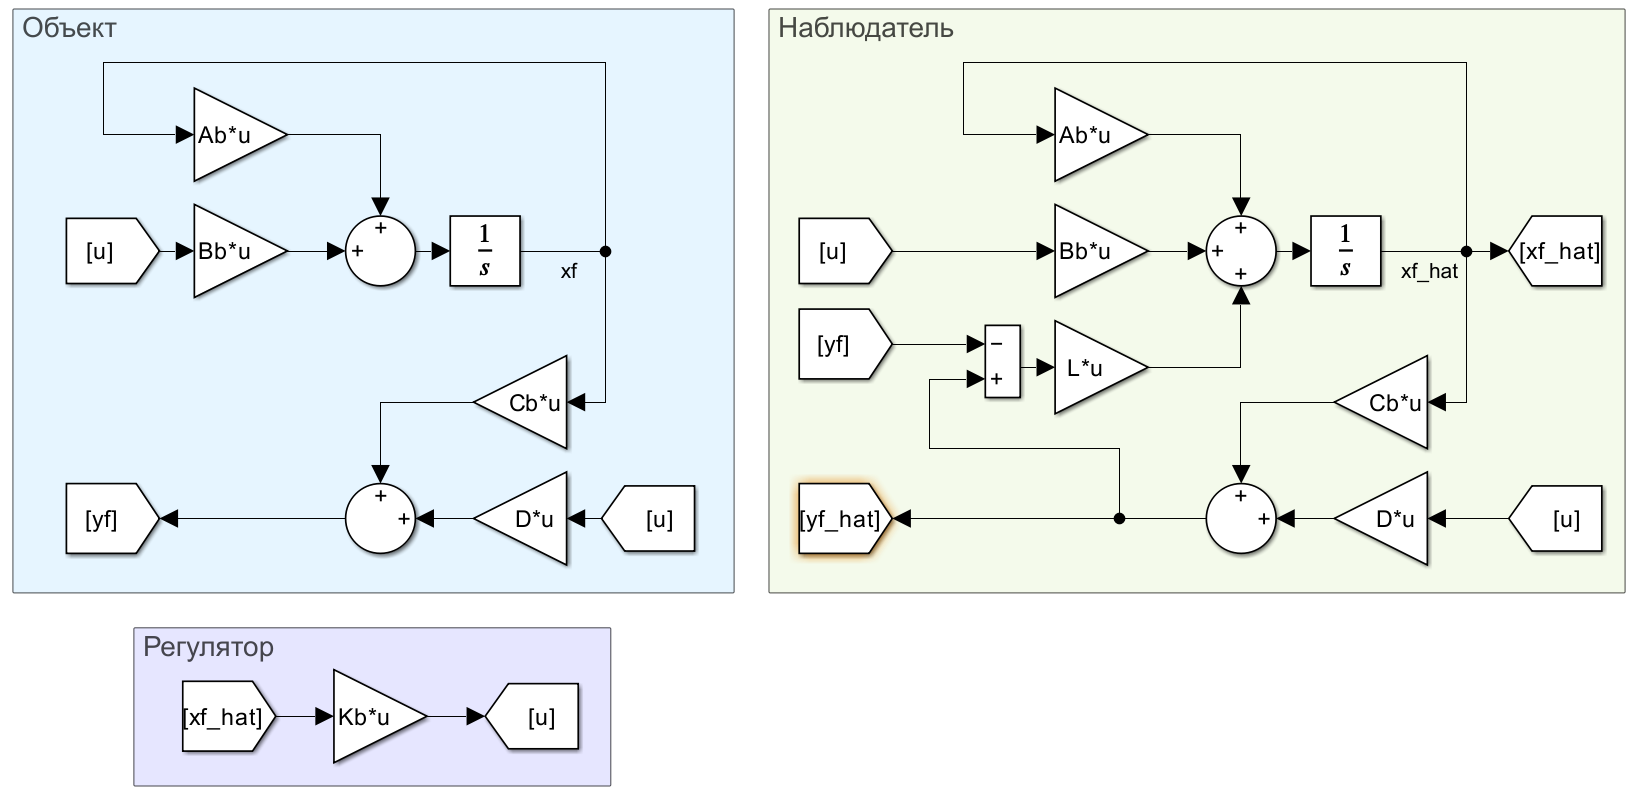
\includegraphics[width=\linewidth]{figs/2slx.png}
    \caption{Схема системы \eqref{eq:sys2} с регулятором \eqref{eq:obs}
    и наблюдателем \eqref{eq:reg}}
    \label{fig:slx}
\end{figure}


\subsection{Синтез «feedback»-компоненты}

Синтезируем «feedback»-компоненту $K$ регулятора \eqref{eq:reg} при 
помощи матричных уравнений типа Сильвестра:
\begin{equation*}
    AP-P\Gamma=BY,\quad K=-YP^{-1}.
\end{equation*}
Проверим условия существования единсвенного невырожденного решения. 
Выберем матрицы:
\begin{equation*}
    \Gamma=\begin{bmatrix}
        -1 & 0 \\ 0 & -2
    \end{bmatrix},\quad
    Y = \begin{bmatrix}
        1 & 1 \\ 1 & 1
    \end{bmatrix}.
\end{equation*}
\begin{enumerate}
    \item Спектры $A$ и $\Gamma$ должны не пересекаться, $\sigma(A)=\{-0.6180,\ 1.6180\}$,
    условие выполняется.
    \item $(A,\ B)$ управляема, проверено в \autoref{sec:anal}.
    \item $(C,\ A)$ наблюдаема, проверено в \autoref{sec:anal}.
    \item Ранг матрицы $BY$ единичный, выполняется:
    \begin{equation*}
        BY=\begin{bmatrix}
            3	&3\\
            5	&5
        \end{bmatrix}.
    \end{equation*}
    \item Произведение матриц $BY$ декомпозируемо на произведение векторов $BY=bh$, 
    для которых выполняется условие полной управляемости $(A,\ b)$ и полной 
    наблюдаемости $(h,\ \Gamma)$, выполняется:
\begin{equation*}
    b=\begin{bmatrix}
        -1.477\\
        -2.462
    \end{bmatrix},\quad
    h=\begin{bmatrix}
        -2.031 & -2.031
    \end{bmatrix},
\end{equation*}
\begin{equation*}
    U_{Ab}=\begin{bmatrix}
        -1.4774&	-2.4624\\
        -2.4624&	-3.9398
    \end{bmatrix},\quad
    V_{h\Gamma}=\begin{bmatrix}
        -2.0305&	-2.0305\\
        2.0305&	4.0611
    \end{bmatrix}.
\end{equation*}
Матрицу полноранговые, значит пара $(A,\ b)$ управляема и  $(h,\ \Gamma)$ наблюдаема.
\end{enumerate}
\noindent Используя CVX получим
\begin{equation*}
    K=\begin{bmatrix}
        -3.0000	&1.0000\\
        -3.0000	&1.0000
    \end{bmatrix}.
\end{equation*}


\subsection{Синтез «feedforward»-компоненты}

Матричные уравнения Франкиса-Дэвисона:
\begin{equation*}
    \begin{cases}
        P\Gamma_w-(A+BK)P-B_fY_1=BK_w\\
        (C_z+D_zK)P+D_zK_w=Y_g
    \end{cases}.
\end{equation*}
Для существования решения необходимо проверить ранги следующих матриц:
\begin{gather*}
    rank\begin{bmatrix}
        A+BK+6iI & B \\
        C_z+D_zK & D_z
    \end{bmatrix}=4,\quad
    rank\begin{bmatrix}
        A+BK-6iI & B \\
        C_z+D_zK & D_z
    \end{bmatrix}=4,\quad
    rank\begin{bmatrix}
        A+BK+3iI & B \\
        C_z+D_zK & D_z
    \end{bmatrix}=4,\quad\\[2ex]
    rank\begin{bmatrix}
        A+BK-3iI & B \\
        C_z+D_zK & D_z
    \end{bmatrix}=4,\quad
    rank\begin{bmatrix}
        A+BK+iI & B \\
        C_z+D_zK & D_z
    \end{bmatrix}=4,\quad
    rank\begin{bmatrix}
        A+BK-iI & B \\
        C_z+D_zK & D_z
    \end{bmatrix}=4.
\end{gather*}
Условие выполняется.
% \begin{enumerate}
%     \item Множество нулей системы $W(s)$ не пересекается со спектром $\Gamma$:
%     \begin{equation*}
%         W=C(sI-A)^{-1}B=\begin{bmatrix}
%             -\dfrac{1.0\,{\left(s-1.0\right)}}{-1.0\,s^2 +s+1.0} & -\dfrac{2.0}{-1.0\,s^2 +s+1.0}\\[2ex]
%             \dfrac{3.0\,s+4.0}{-1.0\,s^2 +s+1.0} & \dfrac{2.0\,{\left(7.0\,s+3.0\right)}}{-1.0\,s^2 +s+1.0}
%         \end{bmatrix},
%     \end{equation*}
%     \begin{equation*}
%         \Delta W=\dfrac{14}{-s^2 +s+1},
%     \end{equation*}
%     получается, что у системы нет нулей, так что условие выполняется.
%     \item Система $W(s)$ полностью управляема по выходу - проверено в \autoref{sec:anal}.
%     \item Количество входов равно или больше количества выходов системы - в данной системе
%     они равны.
%     \item  Если количество входов равно количеству выходов, то система $W(s)$ должна быть 
%    невырожденной - по определителю выше видно, что условие выполняется.
% \end{enumerate}
Используя CVX получим решение
\begin{equation*}
    K_w=\begin{bmatrix}
        1.846 & 0.9709 & 0.9207 & -1.103 & 0.7236 & -6.236\\
        -0.2012 & 0.6522 & -3.377 & 9.979 & 4.781 & -9.777
    \end{bmatrix}.
\end{equation*}

\subsection{Синтез наблюдателя}

Наблюдатель \eqref{eq:obs} синтезируем с помощью уравнения Сильвестра:
\begin{equation*}
    Q\bar A-\Gamma Q=Y\bar C,\quad L=-Q^{-1}Y.
\end{equation*}
Выберем следующие матрицы:
\begin{equation*}
    \Gamma=\begin{bmatrix}
        -1 & 0 & 0 & 0 & 0 & 0 & 0 & 0\\
        0 & -2 & 0 & 0 & 0 & 0 & 0 & 0\\
        0 & 0 & -3 & 0 & 0 & 0 & 0 & 0\\
        0 & 0 & 0 & -4 & 0 & 0 & 0 & 0\\
        0 & 0 & 0 & 0 & -5 & 0 & 0 & 0\\
        0 & 0 & 0 & 0 & 0 & -6 & 0 & 0\\
        0 & 0 & 0 & 0 & 0 & 0 & -7 & 0\\
        0 & 0 & 0 & 0 & 0 & 0 & 0 & -8
    \end{bmatrix},\quad
    Y=\begin{bmatrix}
1 & 1\\
1 & 1\\
1 & 1\\
1 & 1\\
1 & 1\\
1 & 1\\
1 & 1\\
1 & 1
    \end{bmatrix}.
\end{equation*}
С помощью CVX найдем $L$:
\begin{equation*}
    L=\begin{bmatrix}
-15.78 & -15.78\\
-17.99 & -17.99\\
-3.875 & -3.875\\
0.8105 & 0.8105\\
1.453 & 1.453\\
1.466 & 1.466\\
56.84 & 56.84\\
52.86 & 52.86
    \end{bmatrix}.
\end{equation*}

\subsection{Компьютерное моделирование}

Выполним компьютерное моделирование замкнутой системы с нулевыми 
начальными условиями наблюдателей. Построим график формируемого регулятором
управления $u(t)$, $g(t)$, графики фактического и виртуального (регулируемого)
выходов $y(t)$ и $z(t)$, графики внешних воздействий $f_1(t)$, $f_2(t)$. 
Их можно увидеть на \autoref{fig:2fig}. 
Сравнительные графики векторов состояния системы $x(t)$ и генератора $w(t)$
и их оценок, а также ошибок оценки e(t) можно уивдеть на 
рисунках \ref{fig:2fig1} и \ref{fig:2fig2}.
\begin{figure}[H]
    \centering
    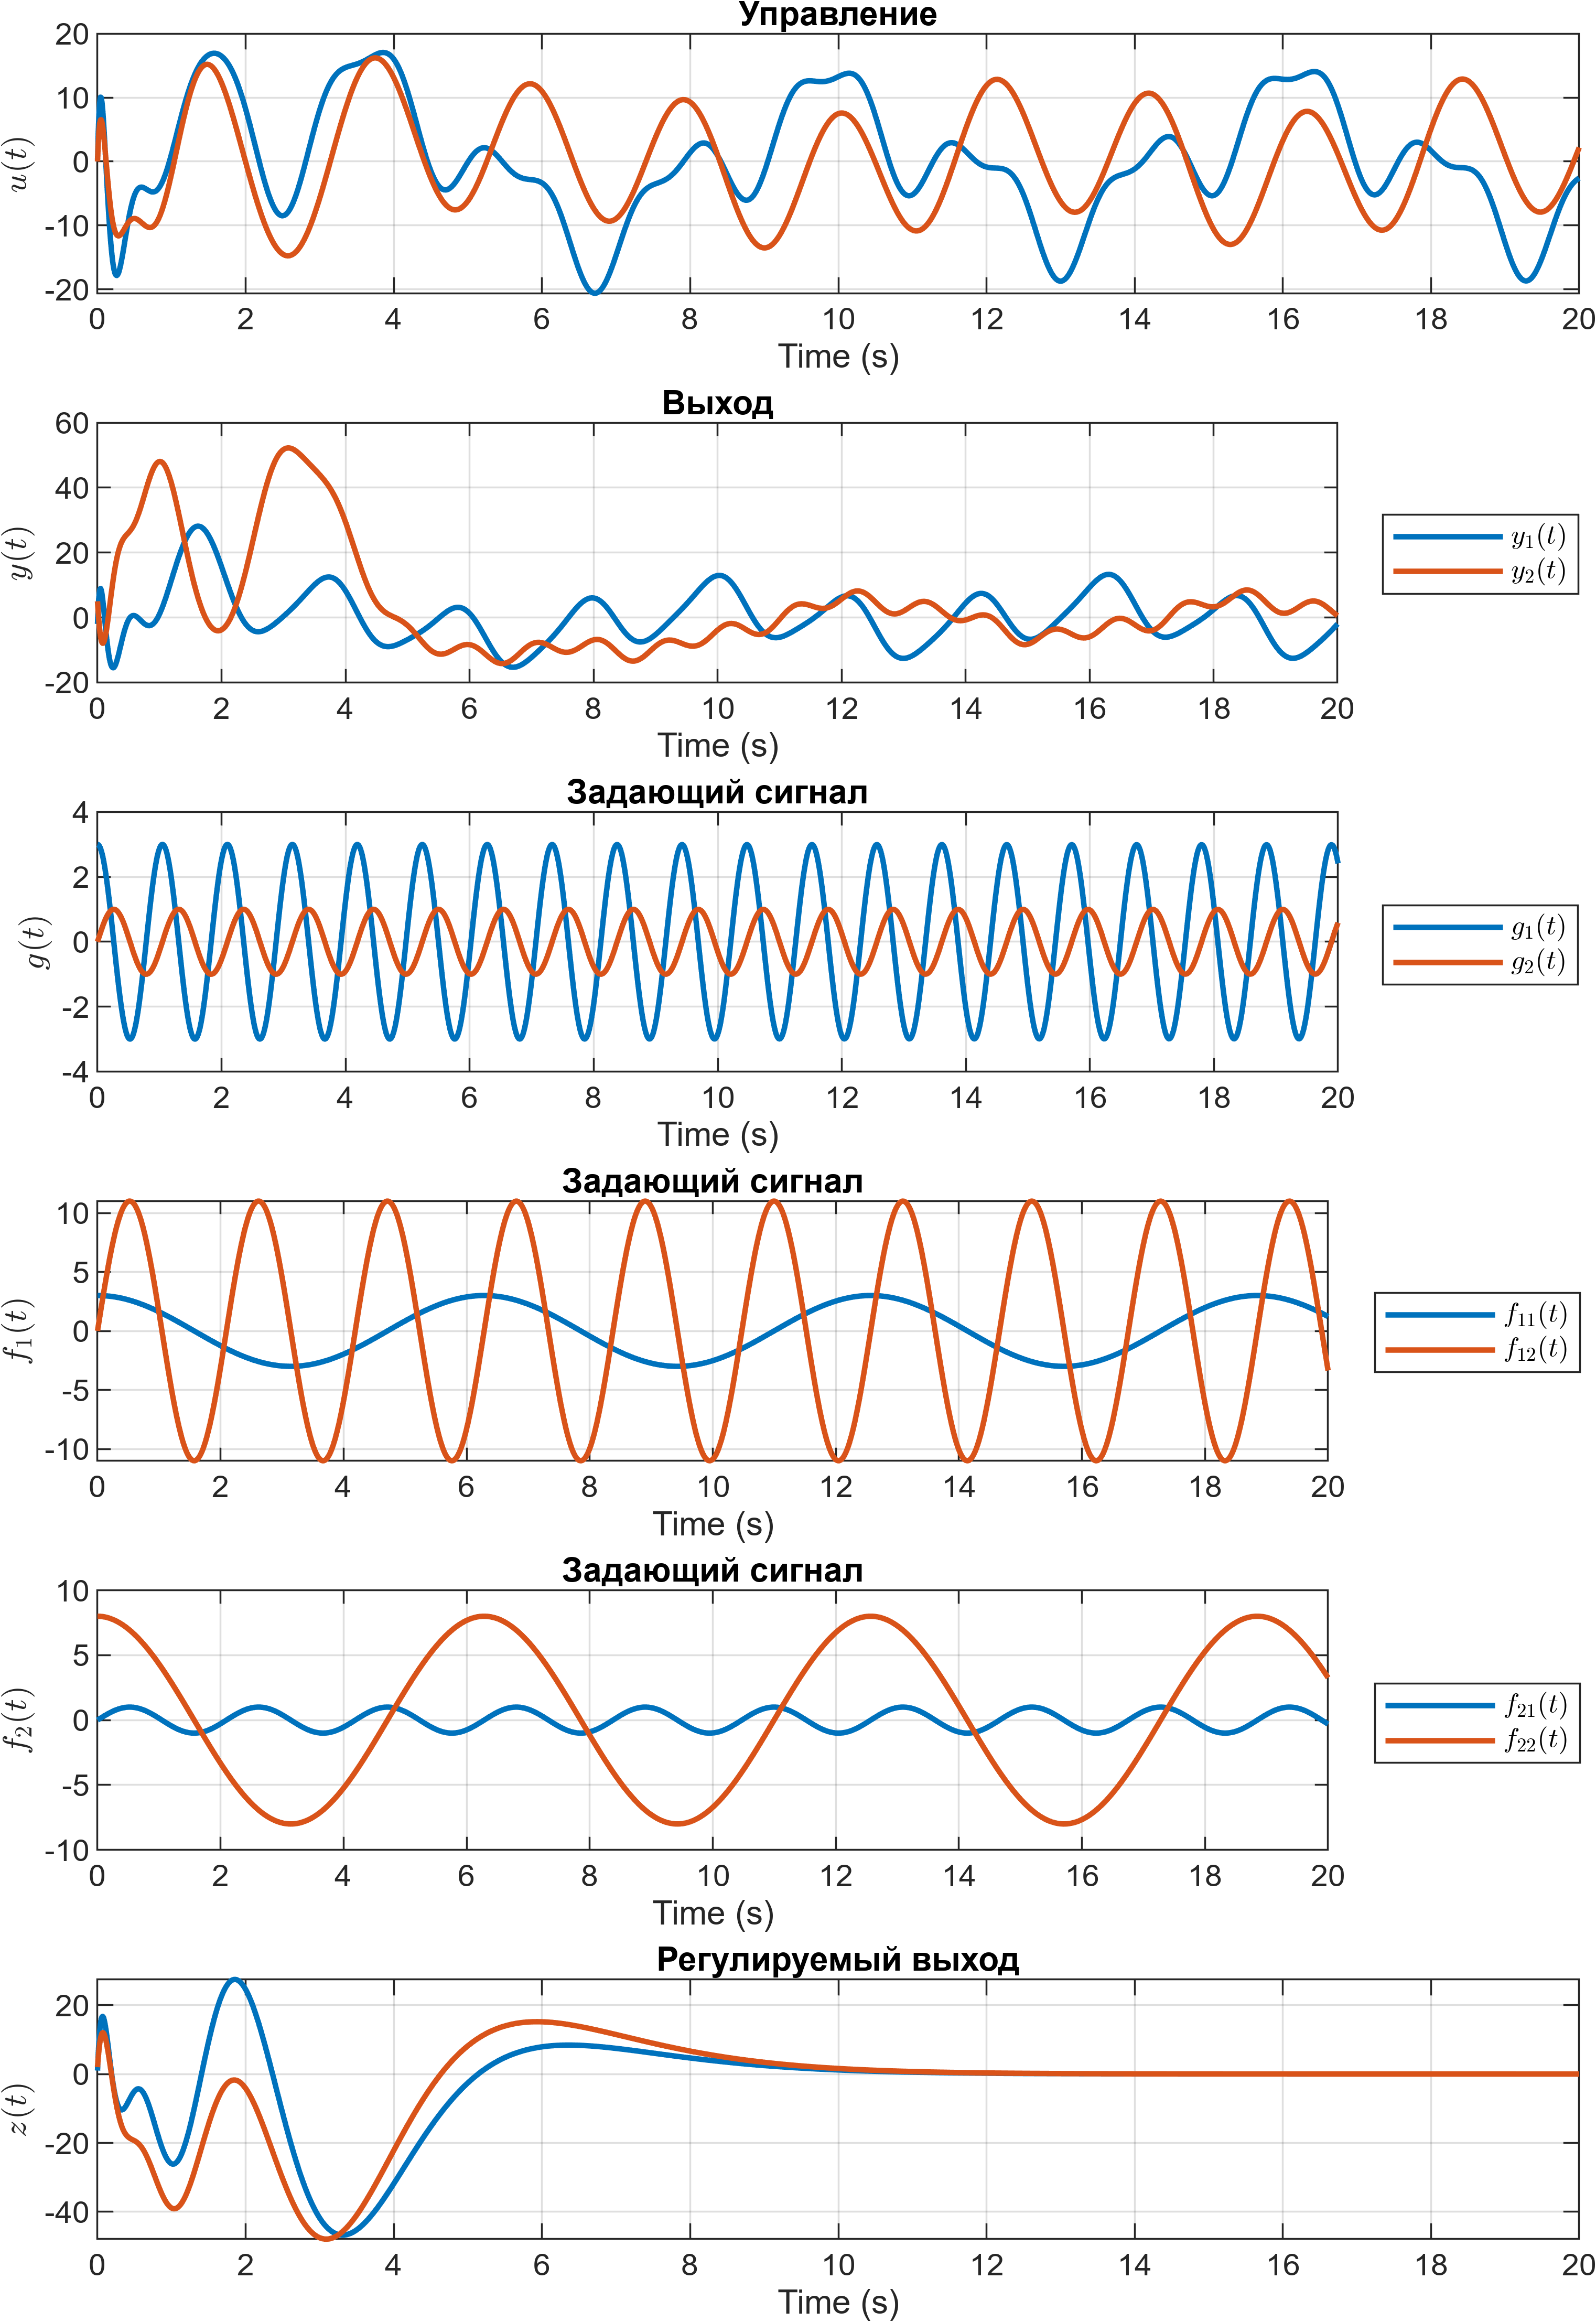
\includegraphics[width=\linewidth]{figs/2fig.png}
    \caption{График формируемого регулятором
    управления $u(t)$, $g(t)$, графики фактического и виртуального (регулируемого)
    выходов $y(t)$ и $z(t)$, графики внешних воздействий $f_1(t)$, $f_2(t)$}
    \label{fig:2fig}
\end{figure}
\begin{figure}[H]
    \centering
    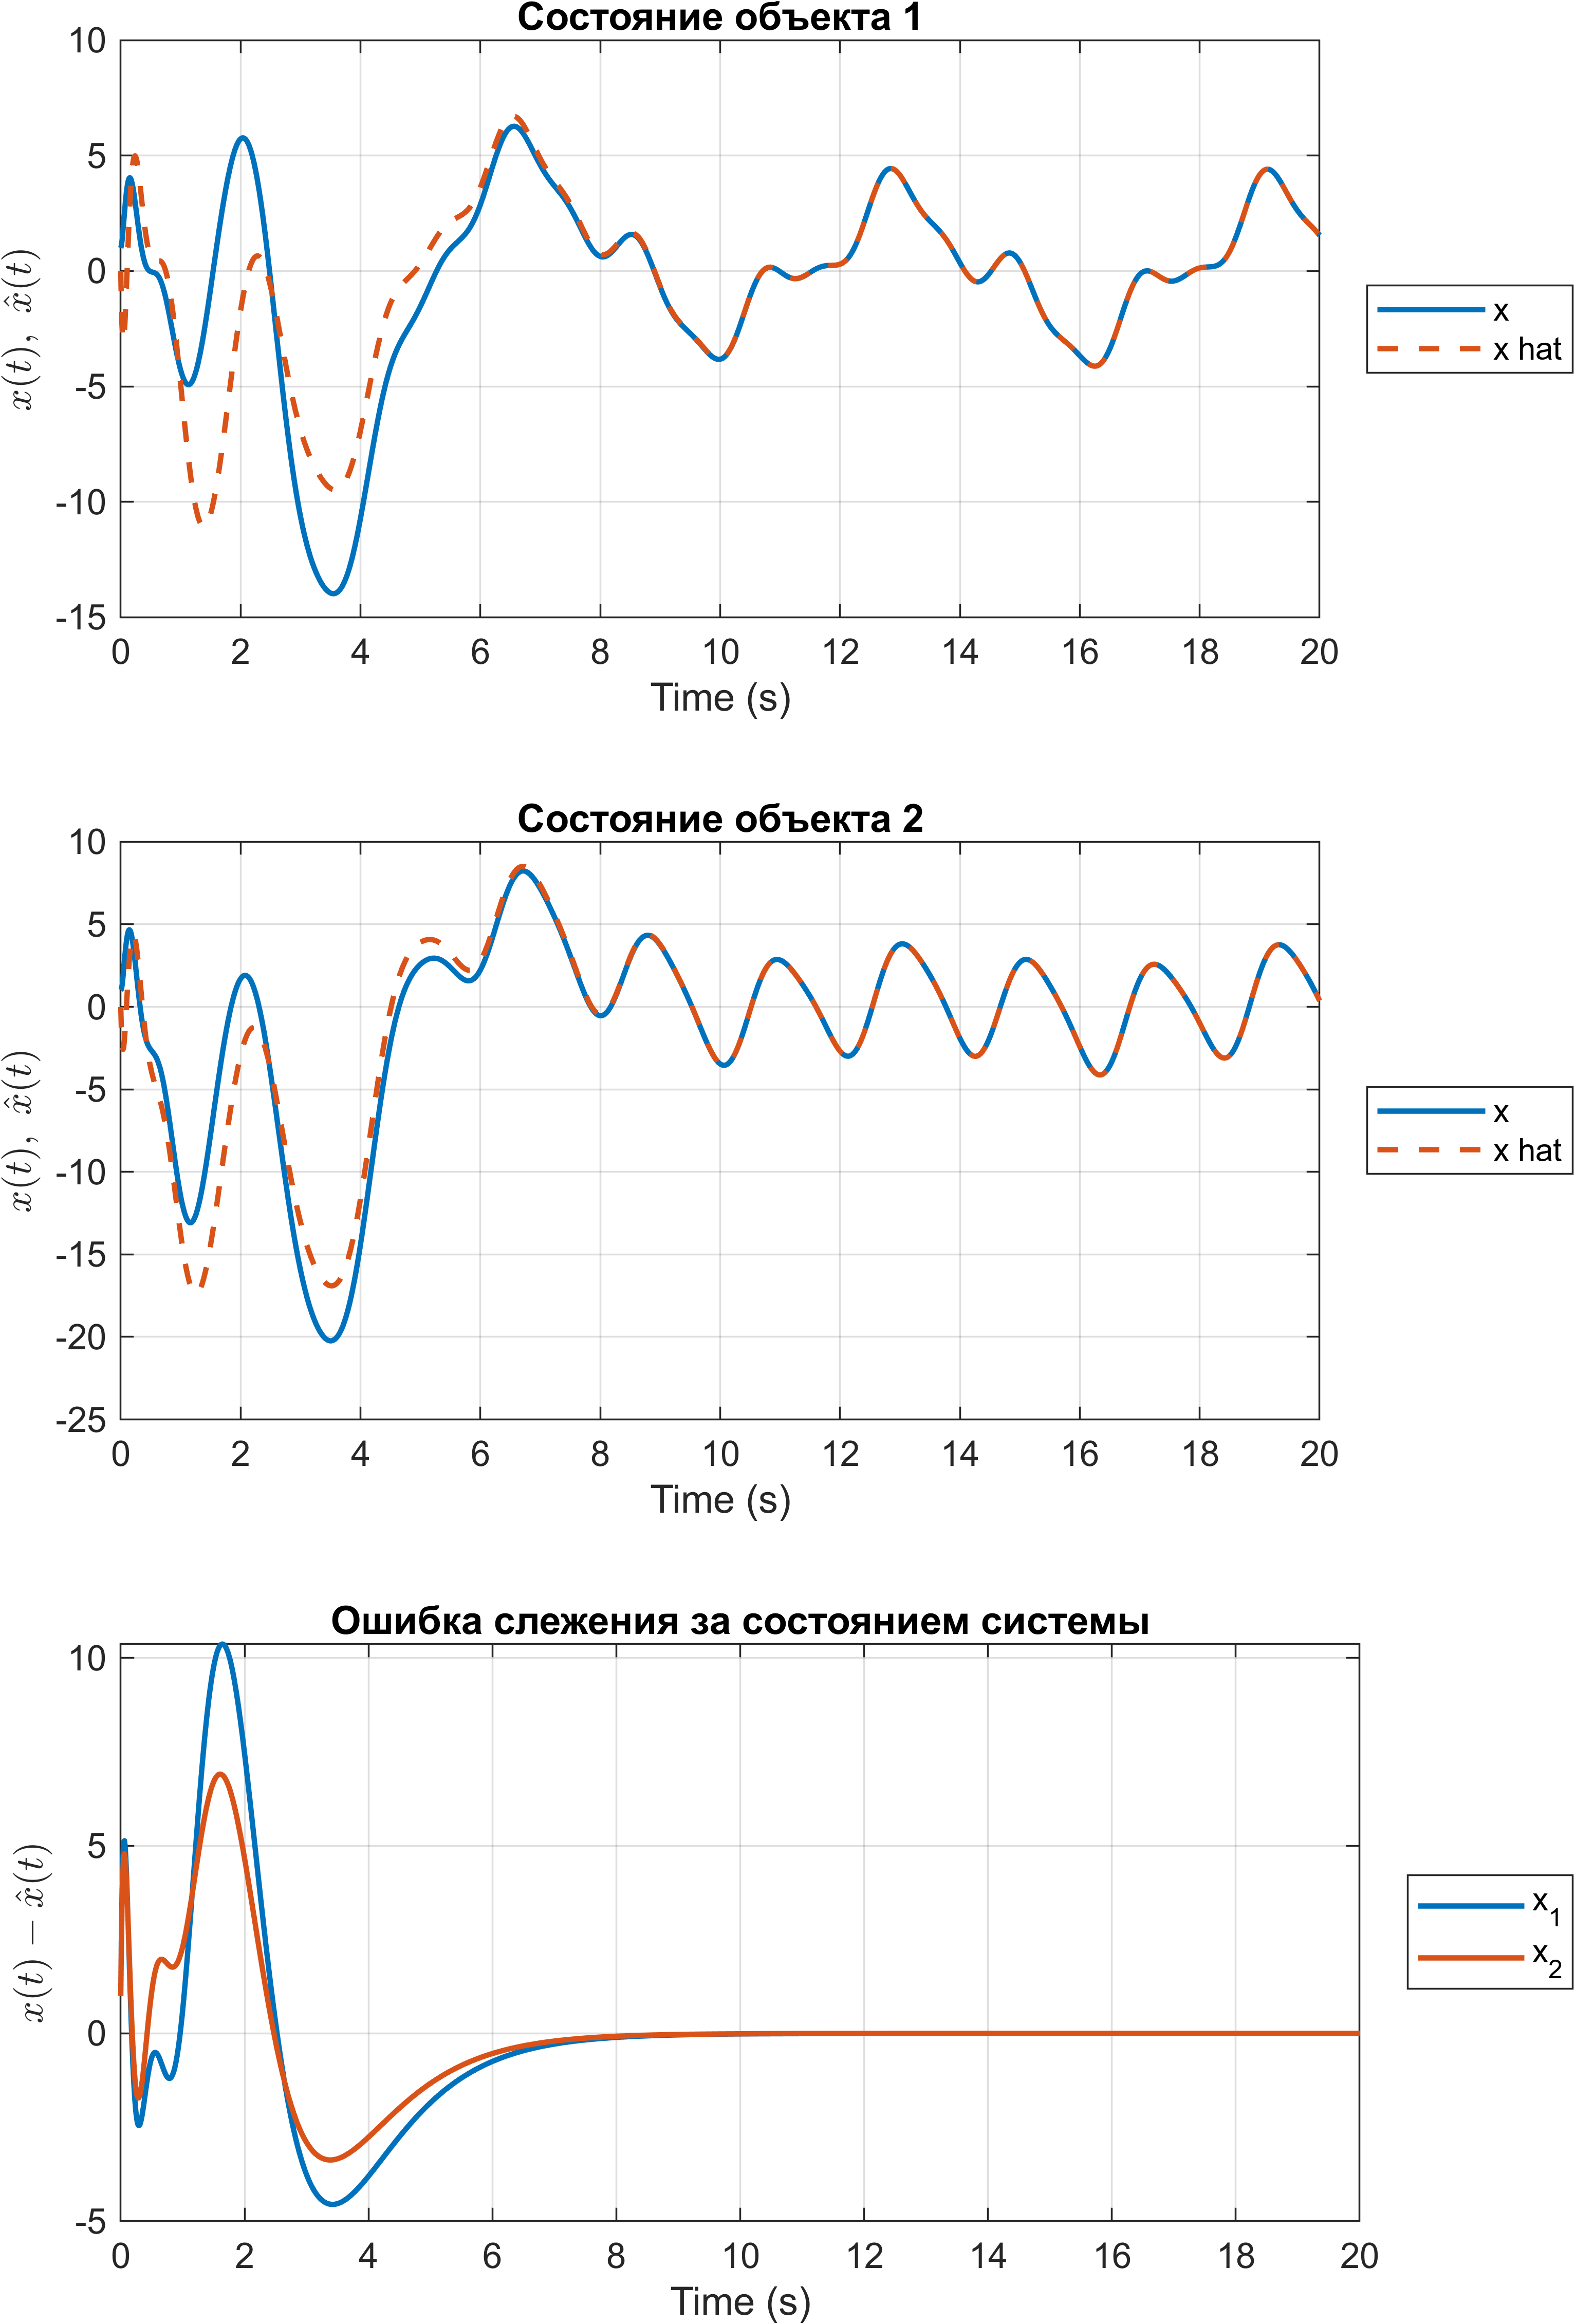
\includegraphics[width=\linewidth]{figs/2fig1.png}
    \caption{Сравнительные графики векторов состояния системы $x(t)$,
    их оценок, а также ошибки оценки}
    \label{fig:2fig1}
\end{figure}
\begin{figure}[H]
    \centering
    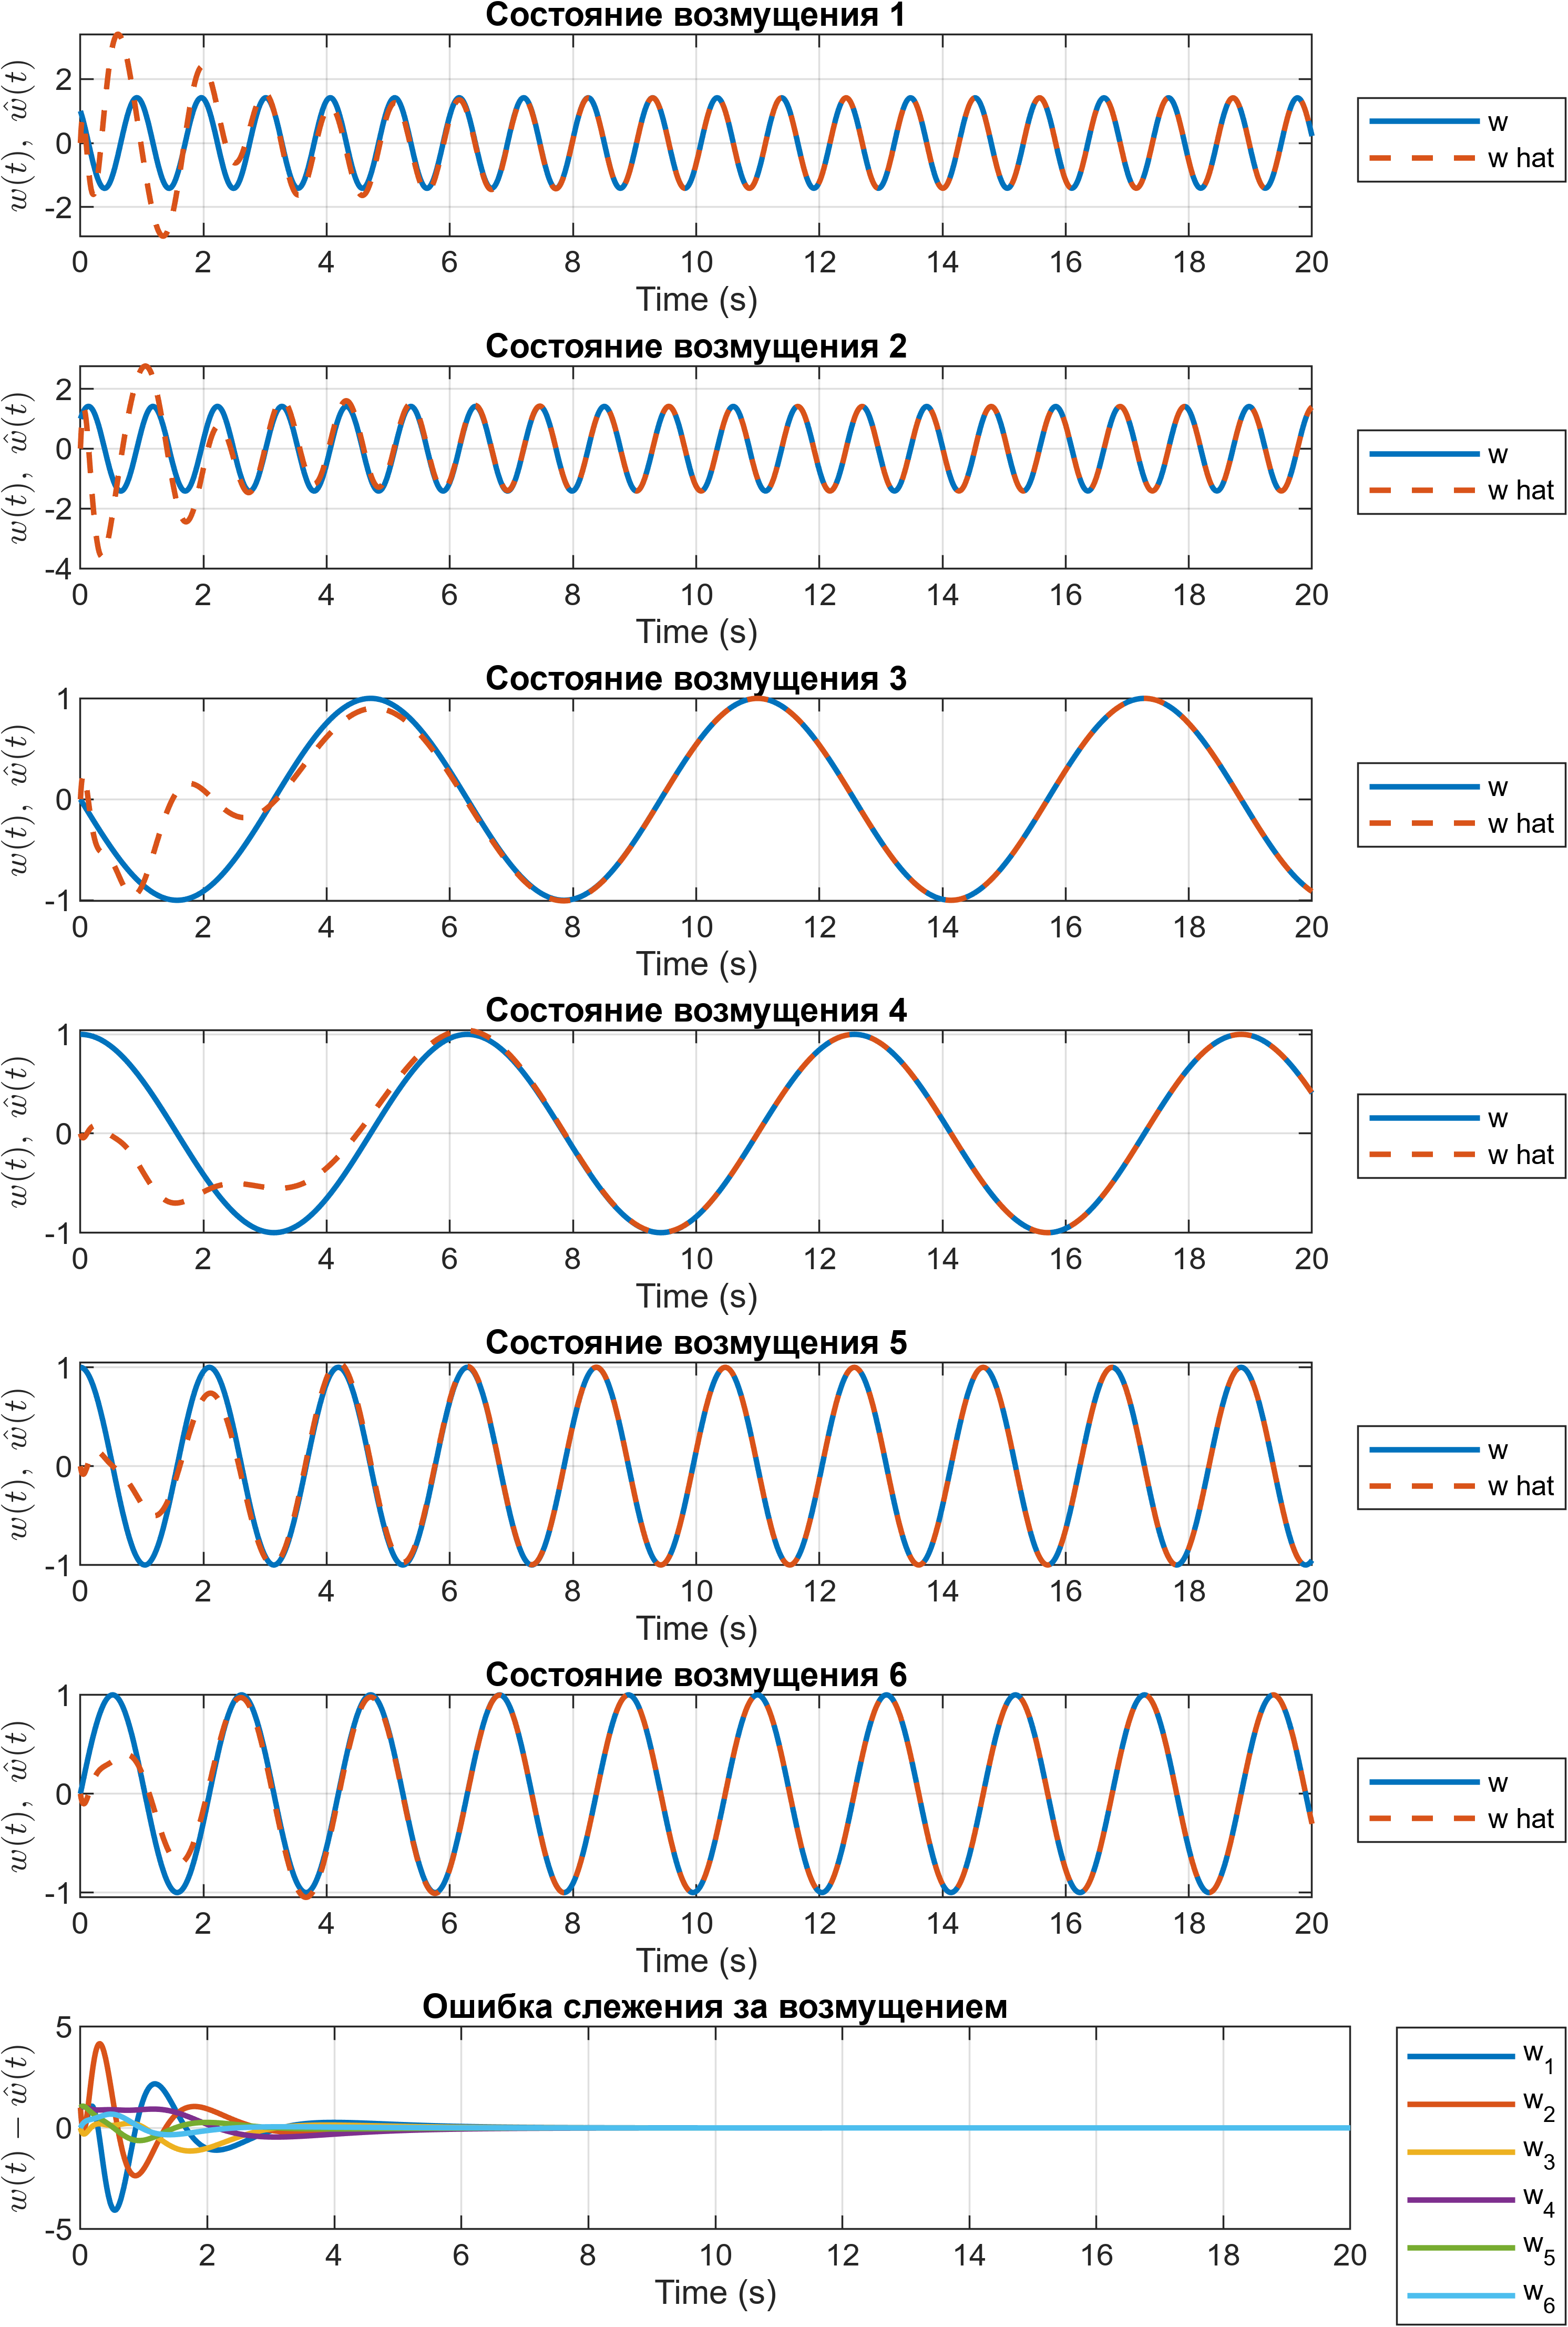
\includegraphics[width=\linewidth]{figs/2fig2.png}
    \caption{Сравнительные графики векторов состояния системы $w(t)$,
    их оценок, а также ошибки оценки}
    \label{fig:2fig2}
\end{figure}

\subsection{Выводы}

Была исследована многоканальная система с внешними 
возмущениями, было показано, что система наблюдаема относительно обоих выходов и 
управлема по состоянию и выходам. 
Были получены «feedback»- и «feedforward»-компоненты регулятора, а также 
синтезирован наблюдатель. Проведенное компьютерное моделирование подтвердило 
выполнение целевого условия $\lim_{t\rightarrow\infty}z(t)=0$, что свидетельствует 
о корректности синтеза. Графики показали, что ошибки оценки состояния системы и 
генератора внешних воздействий стремятся к нулю. 
Таким образом, поставленная задача слежения и компенсации управления успешно решена.


\section{Заключение}

В данной лабораторной работе были исследованы многоканальные системы, а так же решена
задача слежения и компенсации, для этого был синтезировал регулятор на с feedback
и feedforward компонентами на оценках состояния системы и возмущения.
Компьютерное моделирование подтвердило корректность синтеза, показав выполнение
целевого условия и стремление ошибок оценок к нулю.